%===============================================================================
% LaTeX sjabloon voor de bachelorproef toegepaste informatica aan HOGENT
% Meer info op https://github.com/HoGentTIN/latex-hogent-report
%===============================================================================

\documentclass[dutch,dit,thesis]{hogentreport}

\usepackage{lipsum} % For blind text, can be removed after adding actual content

\usepackage{subcaption} % For subfigures

%% Pictures to include in the text can be put in the graphics/ folder
\graphicspath{{../graphics/}}

%% For source code highlighting, requires pygments to be installed
%% Compile with the -shell-escape flag!
%% \usepackage[chapter]{minted}
%% If you compile with the make_thesis.{bat,sh} script, use the following
%% import instead:
\usepackage[chapter,outputdir=../output]{minted}
\setminted[python]{breaklines}

\usemintedstyle{solarized-light}


%% Formatting for minted environments.
\setminted{%
    autogobble,
    frame=lines,
    breaklines,
    linenos,
    tabsize=4
}

%% Ensure the list of listings is in the table of contents
\renewcommand\listoflistingscaption{%
    \IfLanguageName{dutch}{Lijst van codefragmenten}{List of listings}
}
\renewcommand\listingscaption{%
    \IfLanguageName{dutch}{Codefragment}{Listing}
}
\renewcommand*\listoflistings{%
    \cleardoublepage\phantomsection\addcontentsline{toc}{chapter}{\listoflistingscaption}%
    \listof{listing}{\listoflistingscaption}%
}

% Other packages not already included can be imported here
\newcommand{\source}[1]{\caption*{Bron: {#1}} }

%%---------- Document metadata -------------------------------------------------
\author{Ilian Bronchart}
\supervisor{Dhr. B. Van Vreckem}
\cosupervisor{Dhr. J. Campens}
\title[]%
    {Objectherkenning en Datavisualisatie van Observaties met Tobii Eyetracking Glasses in Zorgsimulaties.}
\academicyear{\advance\year by -1 \the\year--\advance\year by 1 \the\year}
\examperiod{1}
\degreesought{\IfLanguageName{dutch}{Professionele bachelor in de toegepaste informatica}{Bachelor of applied computer science}}
\partialthesis{false} %% To display 'in partial fulfilment'
%\institution{Internshipcompany BVBA.}

%% Add global exceptions to the hyphenation here
\hyphenation{back-slash}

%% The bibliography (style and settings are  found in hogentthesis.cls)
\addbibresource{bachproef.bib}            %% Bibliography file
\addbibresource{../voorstel/voorstel.bib} %% Bibliography research proposal
\defbibheading{bibempty}{}

%% Prevent empty pages for right-handed chapter starts in twoside mode
\renewcommand{\cleardoublepage}{\clearpage}

\renewcommand{\arraystretch}{1.2}

%% Content starts here.
\begin{document}

%---------- Front matter -------------------------------------------------------

\frontmatter

\hypersetup{pageanchor=false} %% Disable page numbering references
%% Render a Dutch outer title page if the main language is English
\IfLanguageName{english}{%
    %% If necessary, information can be changed here
    \degreesought{Professionele Bachelor toegepaste informatica}%
    \begin{otherlanguage}{dutch}%
       \maketitle%
    \end{otherlanguage}%
}{}

%% Generates title page content
\maketitle
\hypersetup{pageanchor=true}

%%=============================================================================
%% Voorwoord
%%=============================================================================

\chapter*{\IfLanguageName{dutch}{Woord vooraf}{Preface}}%
\label{ch:voorwoord}

Toen ik op het forum voor potentiële bachelorproefonderwerpen dit project rond computer visie in het Zorglab zag, was mijn interesse onmiddellijk gewekt. 
Na enkele jaren professioneel actief te zijn in de wereld van computer vision, zag ik hierin een unieke kans om 
mijn technische vaardigheden in te zetten voor een maatschappelijk relevant doel.
Bovendien bood het een gelegenheid om meer te leren over de nuances en valkuilen binnen de zorgverlening – een wereld die tot dan toe relatief onbekend voor me was.

Het zaadje waaruit dit project is gegroeid, werd geplant door dhr. Jorrit Campens, lector en onderzoeker aan HOGENT en een drijvende kracht achter het Zorglab.
Zijn domeinexpertise in de zorg vormde een perfecte aanvulling op mijn technische achtergrond. 
Onze samenwerking voelde als een natuurlijke synergie, waarbij hij me doorheen het hele traject, van gerichte feedback voorzag.
Ik herinner me nog goed ons eerste gesprek in het Zorglab, waarbij dhr. Campens zijn droom schetste van een geautomatiseerde analysemethode voor observaties in zorgsimulaties.
Hij omschreef het toen als `naar de maan gaan', een uitdaging die me meteen aansprak. Voor zijn enthousiasme en stimulans, ben ik hem dan ook bijzonder dankbaar.

Toegegeven, het project was ambitieus en uitdagend, zeker in combinatie met mijn deeltijdse werk als softwareontwikkelaar gedurende het semester.
Desondanks zag ik het als een perfecte kans om de diverse vaardigheden die ik doorheen de jaren heb opgebouwd, samen te brengen.
Mijn IT-reis begon met het ontwikkelen van games in het middelbaar en evolueerde naar het bouwen van webapplicaties en het verkennen van frontend-tecnologieën.
Binnen mijn opleiding aan HOGENT koos ik bewust voor de minor Data \& AI, een domein waarin ik mijn kennis nog verder in wilde verdiepen.
Deze bachelorproef voelde dan ook als een culminatiepunt, waar ik mijn passie voor frontend, backend en data science kon verenigen.

Mijn dank gaat ook uit naar mijn promotor, dhr. Bert Van Vreckem, voor zijn waardevolle inhoudelijke feedback en zijn beschikbaarheid voor overlegmomenten gedurende het traject.
Een speciaal woord van dank wil ik richten aan mijn bonusvader, Dirk Coussement.
Als auteur voor een lokaal blad heeft hij een scherp oog voor taal en heeft hij mij enorm geholpen bij het nalezen van deze bachelorproef.

Tenslotte wil ik ook de studenten bedanken die de tijd namen om deel te nemen aan het experiment in het Zorglab. 
Zonder hun medewerking was het verzamelen van de nodige data niet mogelijk geweest.

Ik hoop dat deze bachelorproef een bruikbare eerste stap vormt naar een meer objectieve en efficiënte manier om observatievaardigheden in zorgopleidingen te evalueren.
%%=============================================================================
%% Samenvatting
%%=============================================================================

\IfLanguageName{english}{%
\selectlanguage{dutch}
\chapter*{Samenvatting}


\selectlanguage{english}
}{}

%%---------- Samenvatting -----------------------------------------------------
% De samenvatting in de hoofdtaal van het document

\chapter*{\IfLanguageName{dutch}{Samenvatting}{Abstract}}

Observatievaardigheden zijn van belang voor zorgverleners, zowel voor accurate diagnoses als voor empathische patiëntondersteuning. 
De huidige evaluatie van deze vaardigheden in gesimuleerde omgevingen steunt vaak op subjectieve 
methoden zoals zelfrapportage en directe observatie door docenten. 
Hoewel de Tobii eyetracking-brillen in het Zorglab van HOGENT objectieve blikdata leveren, 
ontbreekt er tot op heden geschikte software om automatisch te analyseren welke objecten studenten waarnemen en voor hoe lang. 
Deze bachelorproef beantwoordt hoe computervisiemodellen geïntegreerd kunnen worden met 
eyetrackingdata van Tobii Glasses om de observatieprestaties van studenten automatisch te analyseren.
De analyses dienen de feedback door docenten in het Zorglab te versterken.

Deze doelstelling werd uitgewerkt door middel van van een proof-of-concept (PoC) softwareapplicatie. 
Dit proces startte met een literatuurstudie naar eyetracking-analyse en relevante computervisiemodellen (o.a. YOLO, SAM, DINOv2). 
Vervolgens werd een prototype applicatie ontworpen en geïmplementeerd (Python, FastAPI, HTMX), 
inclusief een semi-automatische labeling-tool die gebruik maakt van SAM2 voor objectsegmentatie en -tracking. 
Om de PoC te valideren, werd een gecontroleerd experiment uitgevoerd in het Zorglab. 
Hier genereerden studenten aan de hand van Tobii Pro Glasses 3, eyetrackingopnames tijdens gesimuleerde observatietaken. 
Deze opnames, samen met twee specifieke kalibratieopnames, werden gelabeld met de ontwikkelde tool om een grondwaarheidsdataset te creëren. 
Een analysepijplijn werd ontworpen en geëvalueerd. In deze analyse werd de trackingfunctionaliteit van FastSAM gecombineerd met 
blikgestuurde filtering en classificatie van objectsegmenten, middels een getraind YOLOv11-objectdetectiemodel. 
De prestaties werden geëvalueerd aan de hand van precisie, recall en F1-score, na optimalisatie via een grid search van hyperparameters.

Uit de resultaten bleek dat de combinatie van FastSAM-tracking met een YOLOv11-objectdetector (getraind op 1000 samples per klasse) 
de beste prestaties opleverde, met een F1-score van 0.80, een precisie van 0.94 en een recall van 0.70. 
De hoge precisie toont aan dat het systeem met grote zekerheid de correcte objecten identificeert, 
hoewel een significant deel van de fout-positieven in de werkelijkheid correct gedetecteerde objecten bleken te zijn, die niet in de grondwaarheid waren opgenomen. 
De lagere recall wijst erop dat niet alle bekeken objecten consistent werden gedetecteerd, voornamelijk door problemen met kleine, 
transparante objecten en door inconsistenties tussen de FastSAM-segmentaties en de grondwaarheid. 
De FastSAM-tracking bleek de meest beperkende factor in de pijplijn.

Deze bachelorproef levert een werkend PoC en een methodologie op die de haalbaarheid van geautomatiseerde 
analyse van observatievaardigheden aantoont.\\
Het biedt een objectieve, datagestuurde basis om de feedback aan studenten te verbeteren en de effectiviteit van simulatietraining in de zorg te verhogen.
Op deze manier legt het een fundament voor verder onderzoek naar robuustere analysemethoden.

%---------- Inhoud, lijst figuren, ... -----------------------------------------

\tableofcontents

% In a list of figures, the complete caption will be included. To prevent this,
% ALWAYS add a short description in the caption!
%
%  \caption[short description]{elaborate description}
%
% If you do, only the short description will be used in the list of figures

\listoffigures

% If you included tables and/or source code listings, uncomment the appropriate
% lines.
\listoftables

\listoflistings

% Als je een lijst van afkortingen of termen wil toevoegen, dan hoort die
% hier thuis. Gebruik bijvoorbeeld de ``glossaries'' package.
% https://www.overleaf.com/learn/latex/Glossaries

%---------- Kern ---------------------------------------------------------------

\mainmatter{}

% De eerste hoofdstukken van een bachelorproef zijn meestal een inleiding op
% het onderwerp, literatuurstudie en verantwoording methodologie.
% Aarzel niet om een meer beschrijvende titel aan deze hoofdstukken te geven of
% om bijvoorbeeld de inleiding en/of stand van zaken over meerdere hoofdstukken
% te verspreiden!

%%=============================================================================
%% Inleiding
%%=============================================================================

\chapter{\IfLanguageName{dutch}{Inleiding}{Introduction}}%
\label{ch:inleiding}

Observatievaardigheden van zorgverleners zijn niet enkel belangrijk om nauwkeurige diagnoses te stellen, maar ook om de patiënt te ondersteunen en te begeleiden. 
Zo zien we dat studenten in de ouderenzorg vaak moeite hebben met sociale omgang en communicatie met ouderen. 
In het 360° Zorglab aan HOGENT worden studenten getraind via simulaties waarbij ze in een omgeving zoals een ziekenhuis kamer of woonkamer geplaatst worden.
Zo leren ze de nuances van zorgverlening kennen en worden ze geconfonteerd met concrete situaties. 
Een belangrijk aspect van deze training is dat studenten leren om kritische objecten, zoals een colafles op het nachtkastje van een diabetespatiënt, op te merken.
Tot op heden wordt er gesteund op zelfrapportage en observatie door docenten om de vaardigheden van de sudenten te evalueren.
Echter is dit een subjectieve methode die niet altijd even betrouwbaar is, waardoor er nood is aan een objectievere methode om observatievaardigheden te evalueren.
Het Zorglab beschikt over een Tobii eyetracking-bril die de oogbewegingen van de studenten kunnen registreren, en een camera bezit die het gezichtsveld van de studenten kan opnemen.
Eerder werk richtte zich op het visualiseren van het pad waarlangs de blik van de studenten beweegt, maar zo steunt de analyse op het herbekijken van elke opname.
Bovendien produceert deze methode geen bruikbare metrieken die de prestaties van de studenten objectief kunnen becijferen.
Hierdoor is er een nood aan een geautomatiseerde methode om de eyetrackingdata te analyseren en te visualiseren, zodat trainers snel inzicht krijgen in de observatieprestaties van studenten.

\section{\IfLanguageName{dutch}{Probleemstelling}{Problem Statement}}%
\label{sec:probleemstelling}

Hoewel de Tobii Glasses bruikbare data opleveren, ontbreekt er momenteel geschikte software om te analyseren of studenten daadwerkelijk naar deze objecten hebben gekeken.
Dit gebrek aan dataverwerking en visualisatie maakt het voor trainers lastig om de observatieprestaties van studenten efficiënt te beeordelen en te verbeteren.
Zonder een geautomatiseerde manier om te detecteren welke specifieke objecten studenten wel of niet hebben waargenomen, wordt het geven van directe feedback een tijdrovend proces. 

\section{\IfLanguageName{dutch}{Onderzoeksvraag}{Research question}}%
\label{sec:onderzoeksvraag}

Hoe kunnen computervisie-modellen geïntegreerd worden met eyetrackingdata van Tobii Glasses om observatieprestaties van studenten in het 360° Zorglab automatisch te analyseren en te visualiseren?
Deze onderzoeksvraag wordt uitgewerkt aan de hand van de volgende deelvragen:
\begin{itemize}
    \item Welke barrières (cognitief, technisch of didactisch) ervaren trainers en studenten bij de huidige, handmatige observatiemethode?
    \item Welke bestaande objectdetectie en segmentatie modellen zijn hiervoor geschikt?
    \item Hoe kan een softwareoplossing ontwikkeld worden voor een gebruiksvriendelijke analyse en visualisatie van de eyetrackingdata?
    \item In welke mate kunnen de modellen en de ontwikkelde software:
        \begin{enumerate}
            \item correct bepalen welke kritische objecten studenten hebben waargenomen?
            \item nauwkeurig meten hoe lang studenten naar deze objecten kijken?
        \end{enumerate}
\end{itemize}

\section{\IfLanguageName{dutch}{Onderzoeksdoelstelling}{Research objective}}%
\label{sec:onderzoeksdoelstelling}

Het doel is om trainers in het Zorglab te ondersteunen bij het analyseren en visualiseren van eyetrackingdata, zodat ze snel inzicht krijgen in de observatieprestaties van studenten en kunnen 
vaststellen of belangrijke objecten tijdens zorgsimulaties zijn waargenomen. Er zullen hiervoor twee metrieken worden berekend: naar welke objecten de studenten kijken en hoe lang ze naar deze objecten kijken.
Hiervoor wordt een proof-of-concept softwareoplossing ontwikkeld die de eyetrackingdata van Tobii Glasses combineert met objectdetectie- en segmentatiemodellen op een gebruiksvriendelijke manier.
Ook wordt er onderzocht hoe accuraat het uiteindelijke systeem is in het berekenen van de metrieken.

\section{\IfLanguageName{dutch}{Opzet van deze bachelorproef}{Structure of this bachelor thesis}}%
\label{sec:opzet-bachelorproef}

% Het is gebruikelijk aan het einde van de inleiding een overzicht te
% geven van de opbouw van de rest van de tekst. Deze sectie bevat al een aanzet
% die je kan aanvullen/aanpassen in functie van je eigen tekst.

De rest van deze bachelorproef is als volgt opgebouwd:

In Hoofdstuk~\ref{ch:stand-van-zaken} wordt een overzicht gegeven van de stand van zaken binnen het onderzoeksdomein, op basis van een literatuurstudie.

In Hoofdstuk~\ref{ch:methodologie} wordt de methodologie toegelicht en worden de gebruikte onderzoekstechnieken besproken om een antwoord te kunnen formuleren op de onderzoeksvragen.

In Hoofdstuk~\ref{ch:ontwikkeling} wordt de ontwikkeling van de proof-of-concept applicatie toegelicht.

In Hoofdstuk~\ref{ch:experiment} wordt het experimenteel onderzoek besproken dat werd uitgevoerd om de proof-of-concept applicatie te evalueren.

In Hoofdstuk~\ref{ch:analyse-en-resultaten} worden de experimentele opnames geanalyseerd en de resultaten besproken.

In Hoofdstuk~\ref{ch:conclusie}, tenslotte, wordt de conclusie gegeven en een antwoord geformuleerd op de onderzoeksvragen. Daarbij wordt ook een aanzet gegeven voor toekomstig onderzoek binnen dit domein.
\chapter{\IfLanguageName{dutch}{Stand van zaken}{State of the art}}%
\label{ch:stand-van-zaken}

% Tip: Begin elk hoofdstuk met een paragraaf inleiding die beschrijft hoe
% dit hoofdstuk past binnen het geheel van de bachelorproef. Geef in het
% bijzonder aan wat de link is met het vorige en volgende hoofdstuk.

% Pas na deze inleidende paragraaf komt de eerste sectiehoofding.

Dit hoofdstuk bevat je literatuurstudie. De inhoud gaat verder op de inleiding, maar zal het onderwerp van de bachelorproef *diepgaand* uitspitten. De bedoeling is dat de lezer na lezing van dit hoofdstuk helemaal op de hoogte is van de huidige stand van zaken (state-of-the-art) in het onderzoeksdomein. Iemand die niet vertrouwd is met het onderwerp, weet nu voldoende om de rest van het verhaal te kunnen volgen, zonder dat die er nog andere informatie moet over opzoeken \autocite{Pollefliet2011}.

Je verwijst bij elke bewering die je doet, vakterm die je introduceert, enz.\ naar je bronnen. In \LaTeX{} kan dat met het commando \texttt{$\backslash${textcite\{\}}} of \texttt{$\backslash${autocite\{\}}}. Als argument van het commando geef je de ``sleutel'' van een ``record'' in een bibliografische databank in het Bib\LaTeX{}-formaat (een tekstbestand). Als je expliciet naar de auteur verwijst in de zin (narratieve referentie), gebruik je \texttt{$\backslash${}textcite\{\}}. Soms is de auteursnaam niet expliciet een onderdeel van de zin, dan gebruik je \texttt{$\backslash${}autocite\{\}} (referentie tussen haakjes). Dit gebruik je bv.~bij een citaat, of om in het bijschrift van een overgenomen afbeelding, broncode, tabel, enz. te verwijzen naar de bron. In de volgende paragraaf een voorbeeld van elk.

\textcite{Knuth1998} schreef een van de standaardwerken over sorteer- en zoekalgoritmen. Experten zijn het erover eens dat cloud computing een interessante opportuniteit vormen, zowel voor gebruikers als voor dienstverleners op vlak van informatietechnologie~\autocite{Creeger2009}.

Let er ook op: het \texttt{cite}-commando voor de punt, dus binnen de zin. Je verwijst meteen naar een bron in de eerste zin die erop gebaseerd is, dus niet pas op het einde van een paragraaf.

\begin{figure}
  \centering
  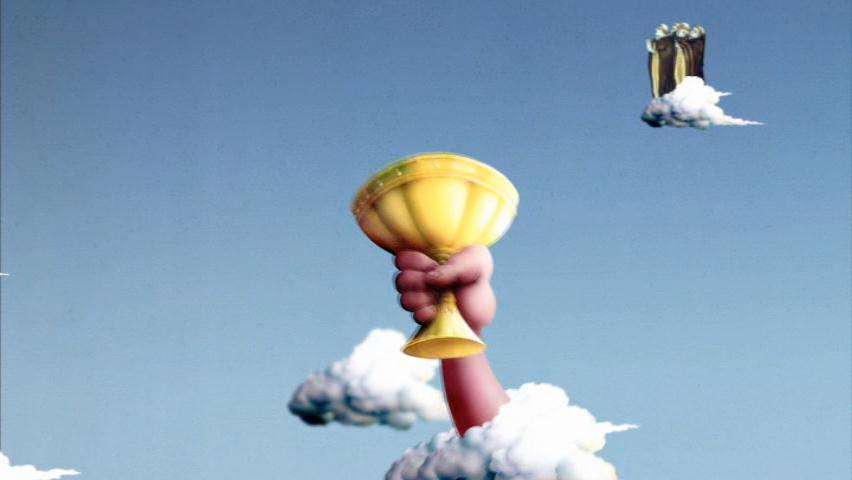
\includegraphics[width=0.8\textwidth]{grail.jpg}
  \caption[Voorbeeld figuur.]{\label{fig:grail}Voorbeeld van invoegen van een figuur. Zorg altijd voor een uitgebreid bijschrift dat de figuur volledig beschrijft zonder in de tekst te moeten gaan zoeken. Vergeet ook je bronvermelding niet!}
\end{figure}

\begin{listing}
  \begin{minted}{python}
    import pandas as pd
    import seaborn as sns

    penguins = sns.load_dataset('penguins')
    sns.relplot(data=penguins, x="flipper_length_mm", y="bill_length_mm", hue="species")
  \end{minted}
  \caption[Voorbeeld codefragment]{Voorbeeld van het invoegen van een codefragment.}
\end{listing}

\lipsum[7-20]

\begin{table}
  \centering
  \begin{tabular}{lcr}
    \toprule
    \textbf{Kolom 1} & \textbf{Kolom 2} & \textbf{Kolom 3} \\
    $\alpha$         & $\beta$          & $\gamma$         \\
    \midrule
    A                & 10.230           & a                \\
    B                & 45.678           & b                \\
    C                & 99.987           & c                \\
    \bottomrule
  \end{tabular}
  \caption[Voorbeeld tabel]{\label{tab:example}Voorbeeld van een tabel.}
\end{table}


%%=============================================================================
%% Methodologie
%%=============================================================================

\chapter{\IfLanguageName{dutch}{Methodologie}{Methodology}}%
\label{ch:methodologie}

Het onderzoek werd uitgevoerd in een iteratieve cyclus, waarbij de verschillende fasen van het project elkaar opvolgden en elkaar beïnvloedden.
Deze sectie beschrijft in grote lijnen de verschillende fasen van het onderzoek, de doelstellingen en de gebruikte methodologieën.
Figuur~\ref{fig:methodologie} toont een flowchart van de methodologie, waarin de verschillende fasen en hun onderlinge relaties worden weergegeven.
De labels op de pijlen geven de belangrijkste deliverables van elke fase aan, die als input dienen voor de volgende fase(s).
\begin{figure}[H]
  \centering
  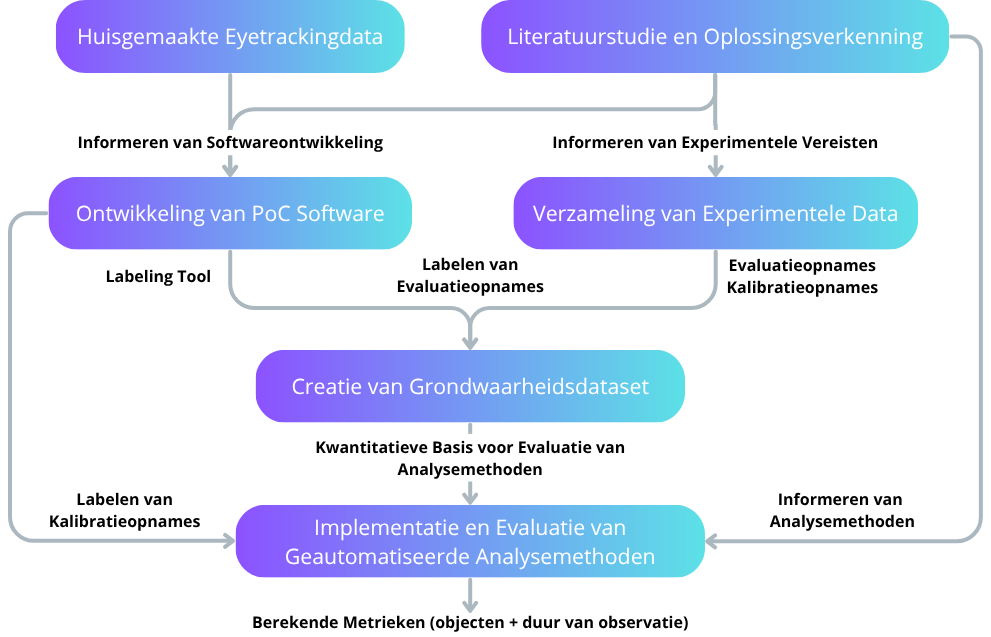
\includegraphics[width=0.9\textwidth]{methodologie.png}
  \caption{Flowchart van de methodologie van het onderzoek.}
  \label{fig:methodologie}
\end{figure}

\section{Literatuurstudie}

De literatuurstudie vormde een iteratief proces gedurende het gehele onderzoek, beginnend met een brede initiële verkenning en 
later verfijnd en aangevuld naarmate specifieke vragen tijdens het project opdoken. 
Het overkoepelende doel was een grondig en actueel inzicht te verwerven in de relevante domeinen. 
Hierbij lag de focus op de volgende gebieden: 
\begin{enumerate}
  \item Onderzoeken hoe de evaluatie van observatieprestaties momenteel wordt uitgevoerd, met bijzondere aandacht aan de nood aan een geautomatiseerde aanpak.
  \item De huidige stand van zaken in eyetracking-technologie, met aandacht voor hoofd-gemonteerde systemen zoals de Tobii Pro Glasses 3 en de analyse van de hieruit voortkomende data.
  \item State-of-the-art technieken binnen Computer Vision, waaronder objectdetectie (bv. YOLO, DETR, Grounding DINO), segmentatie (bv. Mask R-CNN, SAM, FastSAM) en image embedding (bv. CLIP, DINOv2).
  \item Bestaande integraties van eyetracking en Computer Vision.
\end{enumerate}
Wetenschappelijke publicaties, technische documentatie en relevante open-sour\-ce projecten werden hiervoor systematisch 
geraadpleegd en kritisch geanalyseerd.
Hoofdstuk~\ref{ch:stand-van-zaken} beschrijft uitvoerig de bevindingen van deze literatuurstudie.

\section{Oplossingsverkenning}

Voortbouwend op de inzichten uit de literatuurstudie, richtte de tweede fase zich op het verkennen en evalueren van verschillende 
conceptuele oplossingsstrategieën om de centrale onderzoeksvraag te beantwoorden. 
Het doel was om een reeks potentiële benaderingen te formuleren voor het automatisch analyseren 
van eyetrackingdata in combinatie met computervisiemodellen, en hieruit de meest veelbelovende te 
selecteren voor de ontwikkeling van de Proof-of-Concept (PoC). 
Dit proces omvatte het conceptueel ontwerpen van diverse pipelines, waarbij de inputs (eyetracking-opnames, objectdefinities) 
en de gewenste outputs (geobserveerde objecten, observatieduur) als leidraad dienden. 
De strategieën varieerden op vlak van algemene aanpak, de typen computervisiemodellen 
en de rol van de blikdata in het proces. 
Elke strategie werd kwalitatief beoordeeld op criteria zoals verwachte accuraatheid, complexiteit van implementatie, 
computationele vereisten en flexibiliteit. 
Deze analyse resulteerde in een beargumenteerde keuze voor de strategie die als basis diende voor het onderzoek, 
zoals gedetailleerd in Hoofdstuk~\ref{ch:oplossingsstrategieen}.

\section{Huisgemaakte Eyetrackingdata}

Voor het onderzoek en het uitwerken van de PoC software-applicatie, was het belangrijk om zicht te krijgen op de werking van de Eyetracker en de bijhorende software.
Daarom werd deze ontleend uit het Zorglab van HoGent voor een periode van 3 weken. 
Tijdens deze periode werden thuis verschillende opnames gemaakt in een woonkamer met diverse objecten, met de volgende specifieke doelstellingen:
\begin{itemize}
    \item Het leren werken met de Tobii Pro Glasses 3 en de bijhorende software.
    \item Nagaan hoe men de eyetrackingdata kan exporteren naar een bruikbaar formaat via de WiFi-verbinding van de eyetracker.
    \item Een dataset creëren die kan dienen als basis voor het uitwerken van de PoC.
\end{itemize}
Deze opnames werden niet gebruikt voor de uiteindelijke evaluatie van de PoC, aangezien de data afkomstig zijn van tests waarbij de onderzoeker zelf de eyetracker droeg.
Hierdoor is er sprake van mogelijke bias, wat de objectiviteit van de data in het gedrang brengt.

\section{Proof of Concept Software Applicatie}

Een kernonderdeel van deze bachelorproef was de ontwikkeling van een Proof-of-Concept (PoC) softwareapplicatie. 
Het hoofddoel van deze fase was het ontwerpen en implementeren van een werkend prototype dat de beoogde workflow ondersteunt: van het importeren van ruwe eyetracking-opnames tot het genereren van gelabelde data die als basis kan dienen voor analyse. 
De methodologie omvatte de selectie van een passende, moderne technologie-stack (o.a. Python, FastAPI, HTMX, SQLite) gericht op modulariteit en toekomstige uitbreidbaarheid. 
Een significant onderdeel was het ontwerp en de implementatie van een semi-automatische labeling-tool, bedoeld om de efficiëntie van het labelingsproces te verhogen. 
Er werd ingezet op duurzame software-ontwikkelpraktijken zoals type hinting en containerisatie (Docker) om de mogelijkheid tot onderhoud en reproduceerbaarheid te waarborgen. 
De resulterende applicatie, inclusief de architectuur, componenten en technische keuzes, wordt uitvoerig beschreven in Hoofdstuk~\ref{ch:ontwikkeling}.

\section{Experimenteel Onderzoek}

Zoals eerder vermeld, werd de thuisopgenomen dataset niet gebruikt voor de evaluatie van de PoC. 
Om een onbevooroordeelde dataset te verkrijgen en om de modaliteiten van de uitwerking te valideren (bijvoorbeeld: invloed van de afstand tussen de Eyetracker en het object, en de aard van de objecten), werd er een gecontroleerd experiment opgezet in het Zorglab van HoGent.
Het doel van dit experiment was om een dataset te creëren die als grond-waarheid diende voor de metrieken die de PoC berekent (bekeken objecten en tijdsduur).
Op de campus werden studenten van diverse opleidingen gevraagd om deel te nemen aan het experiment.
De 14 resulterende opnames werden daarna gelabeld via de labeling-tool van de PoC, met een manuele kwaliteitscontrole om de betrouwbaarheid van de data te waarborgen.
Voor een uitgebreide beschrijving van het opzet en de uitvoering van het experiment, inclusief de gebruikte methodologieën, wordt verwezen naar Hoofdstuk~\ref{ch:experiment}.

\section{Creatie van een Grondwaarheidsdataset}

Om de prestaties van de geautomatiseerde analysemethoden objectief te kunnen evalueren, was de creatie van een nauwkeurige 
grondwaarheidsdataset noodzakelijk. Het doel van deze fase was om, voor elke evaluatieopname uit het experiment, 
frame-per-frame vast te stellen welke van de 15 gedefinieerde objecten daadwerkelijk door de deelnemer werden bekeken. 
De methodologie startte met het voorbereiden van de ruwe opnamedata (video en blikdata). 
Vervolgens werden de evaluatieopnames gelabeld met behulp van de ontwikkelde labeling-tool (zie Hoofdstuk~\ref{ch:ontwikkeling}).
Hierbij segmenteerde de onderzoeker objecten waar de blik van de deelnemer op rustte, met behulp van het SAM2-model en de trackingfunctionaliteit van de labeling-tool.
Deze initiële segmentaties werden daarna gefilterd op basis van de geregistreerde blikpunten, waarbij een cirkelvormig kijkgebied moest overlappen met het segmentatiemasker. 
Dit resulteerde in een dataset die per frame de bekeken objecten, hun bounding boxes en maskeroppervlakte specificeert. 
De correctheid werd manueel gevalideerd. De gedetailleerde stappen van dit proces zijn beschreven in Hoofdstuk~\ref{ch:grondwaarheid}.

\section{Analyse van Observatieprestaties}

De laatste fase van het onderzoek focuste op het implementeren en evalueren van een geautomatiseerde analysepipeline om observatieprestaties te meten, 
conform de gekozen oplossingsstrategie (Strategie 4 uit Hoofdstuk~\ref{ch:oplossingsstrategieen}). 
Het doel was om automatisch te bepalen welke kritische objecten werden waargenomen en hoe lang, en dit te vergelijken met de grondwaarheidsdataset. 
De methodologie omvatte:
\begin{enumerate}
  \item Het toepassen van ``everything-segmentation'' en tracking met FastSAM op de evaluatieopnames.
  \item Het filteren van de resulterende segmenten op basis van objectgrootte en de geregistreerde 
  blikdata (overlap met het blikpunt), wat resulteerde in de te classificeren object ROIs (Regions of Interest).
  \item Het classificeren van deze ROIs met drie verschillende methoden: 
  \begin{itemize}
    \item Een DINOv2 image embedding model, dat de ROIs omzet naar vectorrepresentaties en deze vergelijkt met een Faiss vector-index van de kalibratieopnames.
    \item Een YOLOv11-classificatiemodel, dat specifiek getraind is op de objecten uit de kalibratieopnames.
    \item Het toepassen van een YOLOv11-objectdetectiemodel, dat de ROIs detecteert en de voorspellingen combineert met de eerdere FastSAM-segmen\-taties.
  \end{itemize}
\end{enumerate}
De prestaties van deze geautomatiseerde analysepipeline werden kwantitatief beoordeeld aan de hand van precisie, 
recall en F1-score ten opzichte van de grondwaarheidsdataset. 
De evaluatie ging echter verder dan deze kernmetrieken. 
Er werd een systematische hyperparameteroptimalisatie via een grid search uitgevoerd en modellen 
getraind met verschillende hoeveelheden data werden vergeleken. 
Bovendien vond een diepgaande analyse plaats van de aard van vals-positieve en vals-negatieve detecties, 
waarbij ook de invloed van factoren zoals objectgrootte werd onderzocht. 
Dit proces, inclusief de gedetailleerde methodologie en resultaten, wordt uitvoerig beschreven in Hoofdstuk~\ref{ch:analyse}.
\chapter{Mogelijke Oplossingsstrategieën}
\label{ch:oplossingsstrategieen}

Bij het ontwerpen van een oplossing voor de gestelde problematiek, is het belangrijk om de 
kernfunctionaliteit van het systeem te beschouwen in termen van zijn inputs en outputs. 
Het systeem dient de eyetracking-opnames als input te verwerken en als output de relevante metrieken te leveren.
Hoewel verschillende strategieën zullen leiden tot een proof-of-concept systeem met verschillende eisen, 
zullen ze allemaal grotendeels voldoen aan dezelfde input-output specificatie.

% TODO: hier een figuur toevoegen die de input-output specificatie visualiseert?

\section{Inputs voor het Systeem}

\subsubsection{Opnames}

De tobii eyetracking-opnamen bevatten verschillende gegevens, waarvan de volgende nuttig zijn voor de 
doeleinden van ons specifieke probleem \autocite{Tobii2023}:
\begin{itemize}
    \item \textbf{Video-opname}: De video-opname van de eyetracking-bril, met een resolutie van 1920x1080 pixels en een framerate van 30 fps (frames per seconde).
    \item \textbf{Blikdata}: De blikdata van de eyetracking-bril, die de coördinaten het blikpunt 
    (het punt gedefinieerd door de samenkomst van de twee ooglijnen) bevat in de vorm van een 2D-coördinaatssysteem.
    Deze worden opgenomen met een frequentie van 50 Hz, wat betekent dat er 50 blikpunten per seconde worden geregistreerd.
    \item \textbf{Metadata}: Metadata van de opname, zoals ID van de opname, naam van de deelnemer, tijdstempel, en andere relevante informatie.
\end{itemize}

Andere gegevens omvatten onder andere data afkomstig van de IMU (Inertial Measurement Unit) van de eyetracker, 
zoals de oriëntatie van de bril, de acceleratie, en metingen van het magnetisch veld rond de bril.
Deze kunnen eventueel gebruikt worden als secundaire gegevens voor het verbeteren van de resultaten, 
maar zijn niet noodzakelijk voor de kernfunctionaliteit van het systeem.

\subsubsection{Objecten}

Naast de eyetracking-opnames zelf, vereist het systeem ook een vooraf gedefinieerde lijst van de specifieke objecten waarvan de observatiestatus moet worden bepaald.
Afhankelijk van de gekozen oplossingsstrategie, kan het gaan om een enkele foto van elk object, of een dataset met meerdere beelden (samples) van elk object vanuit verschillende hoeken en onder verschillende belichtingsomstandigheden.

\section{Outputs van het Systeem}

De uiteindelijke doelmetrieken werden eerder gedefinieerd als de specifieke objecten die studenten hebben bekeken en de totale 
tijdsduur van deze observaties per object binnen een opname. 
Deze metrieken zijn echter afgeleide, geaggregeerde waarden die niet rechtstreeks 
uit de ruwe eyetracking-data kunnen worden geëxtraheerd.

Om deze doelmetrieken te kunnen berekenen, moet het systeem eerst een meer fundamentele, primaire output genereren. 
Deze primaire output bestaat, voor elke individuele frame van de video-opname, uit een identificatie van het (de) object(en) 
waarop de blik van de deelnemer op dat specifieke moment gericht was. Met andere woorden, gegeven alle frames uit een opname, 
is het de taak van het systeem om per frame te bepalen welk(e) relevant(e) object(en) zich in het blikveld bevonden en daadwerkelijk werden aangekeken.

Vanuit deze frame-per-frame objectidentificatie kunnen vervolgens de twee beoogde hoofdmetrieken worden afgeleid:
\begin{itemize}
    \item \textbf{Geobserveerde objecten:} Een lijst van alle unieke objecten die gedurende de opname minstens één keer zijn bekeken.
    \item \textbf{Observatieduur per object:} Voor elk geobserveerd object, de cumulatieve tijd (of het aantal frames) die de blik van de deelnemer op dat object gericht was.
\end{itemize}

\section{Oplossingsstrategieën}

De uitdaging is om een systeem te ontwerpen die als brug fungeert tussen de inputgegevens en de outputmetrieken.
Zoals eerder gezien in de stand van zaken, zijn er binnen computervisie verschillende technieken beschikbaar.
Op basis van deze technieken werden verschillende oplossingsstrategieën geformuleerd, elk met hun eigen voor- en nadelen.
Bij elk van deze strategieën is de laatste stap de koppeling van de blikdata aan de objectdetectie-output, 
waarbij enkel de objecten die ook daadwerkelijk bekeken zijn, worden behouden.

\subsection{Strategie 1: Objectdetectie met Vooraf Getrainde Specifieke Modellen}

Deze strategie is gebaseerd op het trainen van een objectdetectiemodel, zoals een variant van YOLO (zie ~\ref{sec:yolo}), 
op de voorgedefiniëerde objecten.

\paragraph{Conceptuele Werking:}
\begin{enumerate}
    \item \textbf{Dataverzameling \& Annotatie}: Er wordt een uitgebreide dataset gecreëerd met beelden van elk te detecteren object. 
    Deze beelden dienen de objecten vanuit verschillende hoeken, onder variërende belichtingscondities en tegen diverse achtergronden te tonen. 
    Elk object in deze trainingsbeelden wordt vervolgens geannoteerd met bounding boxes.
    \item \textbf{Modeltraining}: Een objectdetectiemodel wordt getraind op deze dataset.
    \item \textbf{Analyse van Evaluatieopnames:} Tijdens de analyse van een eyetracking-opname wordt het getrainde model frame-per-frame 
    toegepast op de videobeelden. 
    \item \textbf{Koppeling met Blikdata}
\end{enumerate}

\paragraph{Voordelen:}
\begin{itemize}
    \item \textbf{Snelheid tijdens Analyse:} Zoals vermeld in de stand van zaken, zijn YOLO-modellen geoptimaliseerd voor snelheid.
    \item \textbf{Eenvoudige Analyse:} Deze methode maakt gebruik van een enkel model, tegenover andere strategieën die meerdere modellen combineren.
\end{itemize}

\paragraph{Nadelen:}
\begin{itemize}
    \item \textbf{Dataverzameling:} Het creëren van een dataset met voldoende variatie in objecten en annotaties kan tijdrovend zijn.
    \item \textbf{Modeltraining:} Het trainen van een model vereist aanzienlijke rekenkracht en tijd.
\end{itemize}

\subsection{Strategie 2: Zero-Shot Objectdetectie en Tracking}

Deze aanpak maakt gebruik van recente ontwikkelingen in zero-shot objectdetectie, zoals Grounding DINO, gecombineerd met segmentatie- en trackingmodellen zoals SAM 2.

\paragraph{Conceptuele Werking:}
\begin{enumerate}
    \item \textbf{Zero-Shot Detectie:} Een model zoals Grounding DINO wordt gebruikt om objecten in de videoframes te detecteren op basis van tekstuele prompts (bv. de namen van objecten). Dit vereist geen voorafgaande training op de specifieke objecten.
    \item \textbf{Segmentatie en Initialisatie Tracking:} De output van Grounding DINO (bounding boxes en labels) kan worden gebruikt om initiële segmentatiemaskers te verkrijgen, eventueel verfijnd met SAM. Deze maskers dienen als input voor een trackingalgoritme.
    \item \textbf{Object Tracking:} Een model zoals SAM 2, dat videosegmentatie ondersteunt, wordt gebruikt om de gedetecteerde en gesegmenteerde objecten doorheen de videosequentie te volgen.
    \item \textbf{Koppeling met Blikdata}
\end{enumerate}

\paragraph{Voordelen:}
\begin{itemize}
    \item \textbf{Geen Specifieke Training Nodig:} Elimineert de noodzaak voor het verzamelen van een uitgebreide, geannoteerde dataset en het trainen van een specifiek model voor de Zorglab-objecten.
    \item \textbf{Potentieel Hogere Robuustheid en Generaliseerbaarheid:} Foundation models zoals Grounding DINO zijn getraind op zeer grote en diverse datasets, waardoor ze potentieel beter omgaan met variaties in omgeving en objectuiterlijk, en makkelijker generaliseren naar nieuwe objecten.
\end{itemize}

\paragraph{Nadelen:}
\begin{itemize}
    \item \textbf{Filteren van Fout-Positieven:} Zero-shot modellen kunnen soms objecten detecteren die niet relevant zijn (fout-positieven) of incorrecte labels toekennen, wat filtering achteraf noodzakelijk maakt.
    \item \textbf{Computationele Kosten:} Foundation models zijn vaak groter en computationeel intensiever dan gespecialiseerde modellen zoals YOLO.
    \item \textbf{Complexiteit Pipeline:} Het combineren van meerdere modellen (detectie, segmentatie, tracking) kan leiden tot een complexere implementatie en potentiële accumulatie van fouten tussen de modules.
\end{itemize}

\subsection{Strategie 3: Handmatige Initialisatie Gevolgd door Tracking}

Deze strategie minimaliseert de afhankelijkheid van automatische objectdetectie door een menselijke operator de initiële objecten te laten aanwijzen, waarna een trackingalgoritme het overneemt.

\paragraph{Conceptuele Werking:}
\begin{enumerate}
    \item \textbf{Handmatige Initialisatie:} In één of meerdere keyframes van de video klikt een operator handmatig op de te volgen objecten. Deze interactie kan gebruikt worden om een initiële bounding box of segmentatiemasker te genereren, eventueel met hulp van SAM.
    \item \textbf{Object Tracking:} Vanaf deze initiële handmatige definitie wordt een trackingalgoritme (bv. SAM 2 of een traditioneler trackingmodel) ingezet om de objecten door de rest van de video te volgen.
    \item \textbf{Koppeling met Blikdata}
\end{enumerate}

\paragraph{Voordelen:}
\begin{itemize}
    \item \textbf{Hoge Accuraatheid bij Initialisatie:} Hoge accuraatheid bij handmatige annotatie vermindert de kans op fout-positieven.
    \item \textbf{Geen Model Training Nodig:} Elimineert de noodzaak voor het trainen van een detectiemodel.
\end{itemize}

\paragraph{Nadelen:}
Het handmatig initialiseren van objecten in elke video is extreem tijdrovend en schaalt slecht bij een groot aantal opnames.

\subsection{Strategie 4: Blikgestuurde Segmentatie Gevolgd door Classificatie}

Deze strategie stelt de eyetracking-data centraal in het segmentatieproces, waarna diverse modellen kunnen worden toegepast voor classificatie.
Het maakt gebruik van de "segment everything" capaciteit van moderne segmentatiemodellen, waarbij de blikdata vervolgens wordt ingezet om de voor classificatie relevante segmenten te identificeren.

\paragraph{Conceptuele Werking:}
\begin{enumerate}
    \item \textbf{"Segment Everything" en Object Tracking:} Een model zoals SAM 2 of FastSAM wordt toegepast om in elk frame van de video alle potentiële objecten te segmenteren. 
    Deze gesegmenteerde objecten krijgen een unieke identifier en worden over de frames heen getrackt. Dit resulteert in een verzameling van segmentatiemaskers met bijbehorende object-ID's per frame.
    \item \textbf{Koppeling met Blikdata:} Per frame wordt het blikpunt gebruikt om te bepalen welk(e) van de gesegmenteerde en getrackte objecten daadwerkelijk door de deelnemer worden aangekeken. 
    Dit kan bijvoorbeeld door te controleren of het blikpunt binnen een bepaald segmentatiemasker valt, rekening houdend met de inherente onnauwkeurigheid van de eyetracker.
    \item \textbf{Segment Uitsnijden en Classificatie:} Enkel de segmenten die als "aangekeken" zijn geïdentificeerd, worden uit het frame geknipt.
    Deze uitsnedes kunnen vervolgens geclassificeerd worden met verschillende mogelijke modellen.
\end{enumerate}

Hier is het mogelijk om verschillende benaderingen te gebruiken voor de classificatie van de segmenten:
\begin{itemize}
    \item \textbf{Zero-Shot Classificatie:} Zero-shot classificatiemodellen zoals Grounding DINO kunnen worden toegepast op de gesegmenteerde objecten, waardoor geen specifieke training vereist is.
    \item \textbf{Getraind Classificatiemodel:} Een specifiek getraind model kan worden ingezet om de gesegmenteerde objecten te classificeren.
    \item \textbf{Keypoint-gebaseerde Classificatie:} Een keypoint-gebaseerd model, zoals SIFT of ORB, kan worden gebruikt om de segmenten te classificeren op basis van hun visuele kenmerken.
    \item \textbf{Feature-gebaseerde Classificatie:} Voorgetrainde modellen zoals DINOv2 kunnen in combinatie met een vector-database worden gebruikt om de segmenten te classificeren op basis van hun visuele kenmerken.
    Deze modellen genereren een vingerafdruk (feature vector) van elk segment, die vervolgens kan worden vergeleken met een database van gekende objecten.
    \item \textbf{Classificatie met Vision-API}: Voor classificatie kan ook eventueel gebruik gemaakt worden van een bestaande foundation-model gebaseerde computer-vision diensten (Google, OpenAI, ... APIs).
\end{itemize}

\paragraph{Voordelen:}
\begin{itemize}
    \item \textbf{Potentieel Robuustere Segmentatie en Tracking:} Door alle objecten te segmenteren en te tracken, kan het systeem stabieler zijn tegen kortstondige 
    occlusies of snelle blikverschuivingen. Een object dat even niet wordt aangekeken, blijft toch getrackt en kan later opnieuw als "aangekeken" worden geïdentificeerd zonder nieuwe segmentatie-initiatie.
\end{itemize}

\paragraph{Nadelen:}
\begin{itemize}
    \item \textbf{Beheer van Groot Aantal Segmenten:} Het tracken en beheren van ID's voor potentieel veel segmenten per frame kan complex zijn, vooral in drukke omgevingen.
    \item \textbf{Complexe Pipeline:} Het combineren van segmentatie, tracking en classificatie kan leiden tot een complexe implementatie.
    \item \textbf{Trager dan Directe Objectdetectie:} Het toepassen van meerdere modellen (segmentatie/tracking, classificatie) kan de snelheid van de analyse verminderen in vergelijking met een directe objectdetectie-aanpak.
    \item \textbf{Unknown Objecten:} Het systeem zal veel objecten segmenteren die niet relevant zijn voor de analyse, wat kan leiden tot eventuele fout-positieven in de uiteindelijke classificatie.
\end{itemize}

\section{Keuze van de Oplossingsstrategie}

Na een zorgvuldige afweging van de hierboven beschreven strategieën, elk met hun inherente voor- en nadelen, is voor de ontwikkeling van de PoC 
applicatie gekozen voor \textbf{Strategie 4: "Segment Everything" Gevolgd door Blikselectie en Diverse Classificatiemethoden}.

Deze keuze is primair ingegeven door de veelbelovende resultaten uit initiële, exploratieve tests. 
Waar zero-shot objectdetectie (Grounding DINO), in eerste experimenten nog geen consistent robuuste resultaten opleverden 
(met name wat betreft fout-positieven en generalisatie naar sommige van de specifieke Zorglab-objecten), 
toonden de "segment everything" en tracking-capaciteiten FastSAM direct indrukwekkende prestaties.
Veel van de door de eyetracker geregistreerde objecten konden effectief worden gesegmenteerd en gevolgd. 
De uitdaging verschoof daarmee naar het vinden van een betrouwbare methode om deze dynamisch geïdentificeerde segmenten correct te classificeren.

\begin{itemize}
    \item Strategie 1 (Trainen van een Objectdetector) kon op dit punt in het onderzoekproces niet worden overwogen, omdat er nog geen dataset beschikbaar was.
    \item Strategie 3 (Handmatige Initialisatie) werd als te arbeidsintensief en niet schaalbaar voor de beoogde toepassing beschouwd.
\end{itemize}

De gekozen Strategie 4 biedt de flexibiliteit om verschillende classificatietechnieken te exploreren voor de aangekeken segmenten.
Dit maakt een iteratieve ontwikkeling en optimalisatie van de PoC mogelijk zonder de onderliggende pipeline aanzienlijk te hoeven aanpassen.
Hoewel het efficiënt beheren van vele segmenten en de complexiteit van de pipeline potentiële uitdagingen kent, 
wogen de initiële positieve resultaten van de segmentatie- en trackingcomponenten en de modulaire opzet voor de classificatiestap zwaarder in de besluitvorming.
De de PoC applicatie is uitgewerkt in functie van deze gekozen oplossingsstrategie, en zal in het volgende hoofdstuk verder worden toegelicht.
\chapter{Proof-of-Concept Applicatie}
\label{ch:ontwikkeling}

\section{Inleiding}

Dit hoofdstuk dient als een uitgebreide toelichting op de softwareoplossing die binnen deze bachelorproef is ontwikkeld.
Eerst zullen de verschillende componenten van de applicatie worden besproken, gevolgd door een gedetailleerde uitleg over hoe een gebruiker de applicatie kan gebruiken.
Aangezien er rekening gehouden werd met het effectief inzetten van de applicatie in de praktijk, zullen ook de gebruikte technologieën en technische keuzes worden toegelicht.
Zo kan de software bij opeenvolgende bachelorproeven iteratief verder ontwikkeld worden voor nieuwe toepassingen en verbeteringen.

\section{Applicatiecomponenten en Gebruikersinteractie}

De workflow die bedacht werd voor de proof-of-concept applicatie, om van ruwe data naar bruikbare metrieken te gaan, kan als volgt worden samengevat:
\begin{enumerate}
    \item Er worden één of meerdere `kalibratie-opnames' gemaakt met de eyetrackingbril, waarbij elk object dat onderdeel is van het onderzoek, vanuit verschillende hoeken wordt gefilmd.
    \item Ook worden er opnames gemaakt die daarna geanalyseerd worden, waarbij de studenten in de simulatieomgeving met de eyetrackingbril rondlopen.
    \item De opnames worden geïmporteerd in de applicatie via de WiFi-verbinding van de eyetrackingbril.
    \item Men geeft een naam aan de simulatieomgeving (bijvoorbeeld `Zorglab Zorgkamer') binnen de applicatie en defininieert de objecten.
    \item Daarna kan men beginnen met het labelen van de objecten in de kalibratie-opnames via de ingebouwde labeling-tool. De labeling-data dient als een basis voor het trainen of initialiseren van de analysemodellen.
    \item De applicatie is nu in staat de eyetracking-opnames van de studenten te analyseren en de metrieken te visualiseren. Het visualisatiegedeelte werd niet verder uitgewerkt binnen deze bachelorproef omdat er geen betrouwbaar analysemodel kon worden bekomen; maar verder hierover in Hoofdstuk~\ref{ch:experiment}.
\end{enumerate}
De applicatie is dus opgebouwd uit verschillende componenten die samen een stapsgewijs proces vormen. Deze zullen hieronder verder worden toegelicht.

\subsubsection{Opnames Maken}

Voordat de applicatie ontwikkeld kon worden, waren er eerst een aantal video-opnames nodig. 
In deze fase werd de Tobii eyetracking-bril van het Zorglab ontleend om vertrouwd te raken met het maken van opnames. 
Deze opnames werden thuis uitgevoerd en dienden zowel als basis voor de applicatie zelf als voor initiële experimenten met de computer vision-modellen die later zouden worden ingezet in de labelingtool en de analyses.
Om een opname te maken hebben we twee zaken nodig: de eyetracker zelf met bijbehorende accessoires, en een laptop of computer waarop de `Tobii Pro Glasses 3 Controller'\footnote{\url{https://www.tobii.com/products/eye-trackers/wearables/tobii-pro-glasses-3/controller-app}} app is geïnstalleerd.

\begin{figure}[H]
  \centering
  
\includegraphics[width=0.6\textwidth]{placeholder.jpeg}
  \caption[]{\label{fig:todo} TODO: Foto met de benodigdheden: eyetracker, hub, laptop met app zichtbaar (eyetracker niet geconnecteerd), batterijlader, kalibratiekaart
 }
\end{figure}

De eyetracker zelf bestaat uit een hub die stroom levert aan de bril en de opnames opslaat op een SD-kaart. Daarnaast is er de bril zelf die op het hoofd van de gebruiker wordt geplaatst.
De hub heeft een batterij die opgeladen kan worden met de bijgeleverde oplader. 
Eens de bril geconnecteerd is met de hub via de ingebouwde HDMI-kabel en de hub aan staat met een groen LED-lampje, zou er een WiFi-verbinding moeten verschijnen op de laptop of computer.
Deze verbinding start met `TG', gevolgd door het serienummer van de bril. Het wachtwoord voor de verbinding is `TobiiGlasses'. 
Open de Tobii Pro Glasses 3 Controller-app en observeer of het camerabeeld van de bril zichtbaar is in de app.

\begin{figure}[H]
  \centering
  
\includegraphics[width=0.6\textwidth]{placeholder.jpeg}
  \caption[]{\label{fig:todo} TODO: Foto van de app met camerabeeld zichtbaar, en de knoppen om opnames te maken
 }
\end{figure}

Na het invoegen van de naam van de opname (of participant), druk op de knop `Record' om de opname te starten.
Voordat de opname kan starten, zal de app vragen om de bril te kalibreren. 
Dit kan gedaan worden met de bijgeleverde kalibratiekaart, die op armlengte afstand van de bril dient gehouden te worden.
Aan de participant wordt gevraagd om naar de centrale stip op de kaart te kijken, en vervolgens wordt er op de knop `Calibrate' gedrukt.
De app zal nu beginnen met het opnemen van de video, en de participant kan nu vrij rondlopen in de simulatieomgeving.

% TODO: Best-practices toevoegen?

\subsubsection{Importeren van Eyetracking-Opnames}

Zoals eerder vermeld heeft de Tobii eyetracker twee componenten: de bril zelf en een `hub' die stroom levert aan de bril en de opnames opslaat op een SD-kaart.
Het zou dus mogelijk zijn om de opnames via de SD-kaart te importeren, maar dit is niet praktisch omdat de SD-kaart steeds uit de hub dient gehaald te worden.
Daarom biedt de hub ook een WiFi-verbinding aan, zodat de opnames via een netwerkverbinding kunnen worden geïmporteerd. 

Wanneer men de proof-of-concept applicatie opent op de pagina `Browse Recordings' via de navigatiekolom, worden er twee tabellen getoond (zie figuur \ref{fig:browse-recordings})

\begin{figure}[H]
  \centering
  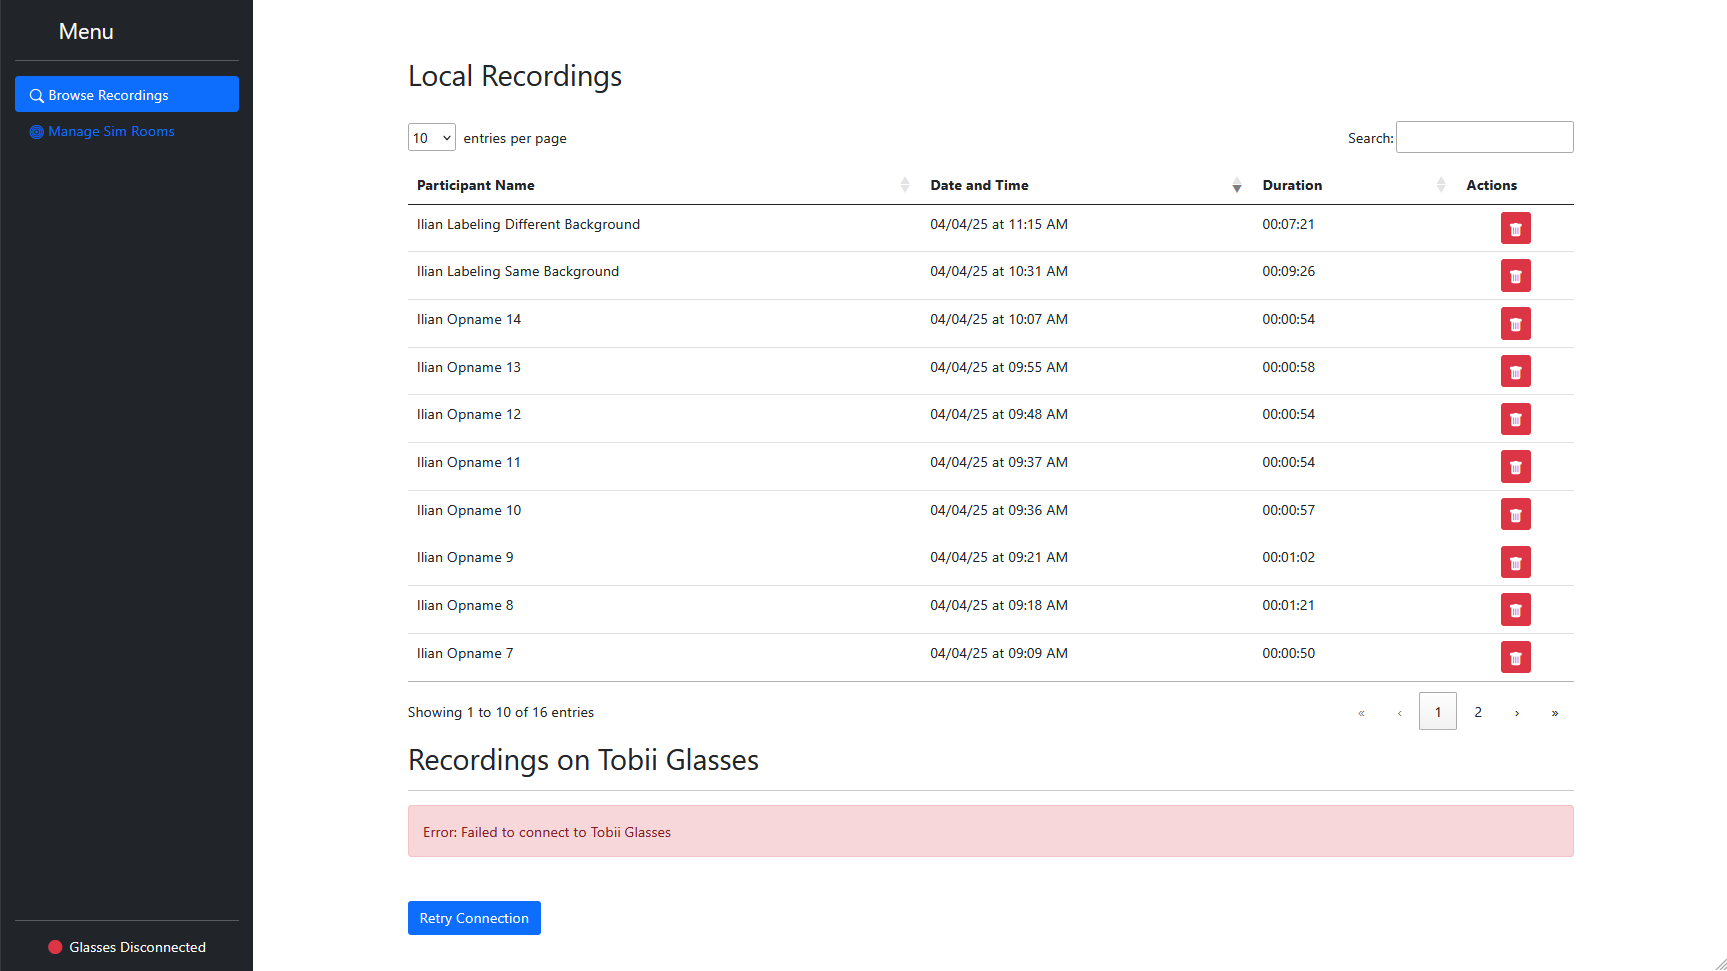
\includegraphics[width=1\textwidth]{browse-recordings.png}
  \caption[]{\label{fig:browse-recordings} Screenshot van de `Browse Recordings'-pagina waar opnames kunnen worden geïmporteerd. Hier is de bril niet verbonden met de computer. }
\end{figure}


De bovenstaande tabel `Local Recordings' toont de opnames die lokaal zijn opgeslagen op de computer, en de onderste tabel `Recordings on Tobii Glasses' toont de opnames die zijn opgeslagen op de hub.
Indien een tabel geen opnames bevat, wordt er een passend bericht getoond.
De opnames worden getoond in tabellen met de naam van elke opname, de datum en tijd waarop deze werd gemaakt, evenals de duur van de opname. 
Het is mogelijk om opnames te verwijderen uit de `Local Recordings'-tabel door op de rode knop met het prullenbakje te klikken naast een opname. Dit heeft geen invloed op de opnames die zijn opgeslagen op de hub.
Ook kan men zoeken naar opnames via de zoekbalk bovenaan de tabellen, en kan men ze sorteren op naam, datum of duur door op de bijbehorende kolomkop te klikken.

Wanneer de bril niet verbonden is met de computer, wordt er een aangepaste melding getoond, met een knop om opnieuw te verbinden. Figuur \ref{fig:browse-recordings} toont een voorbeeld van de interface van de applicatie, waar de bril niet verbonden is met de computer.
Linksonder in de interface toont de applicatie de huidige status van de verbinding met de bril, inclusief de batterijstatus. Bij figuur \ref{fig:browse-recordings-connected} is de bril wel verbonden met de computer. 
Elke rij in de onderste tabel bevat een blauwe knop met een pijl naar beneden, waarmee een opname kan worden geïmporteerd vanuit de bril naar de computer. Dit kan enige tijd duren, afhankelijk van de grootte van de opname.

\begin{figure}[H]
  \centering
  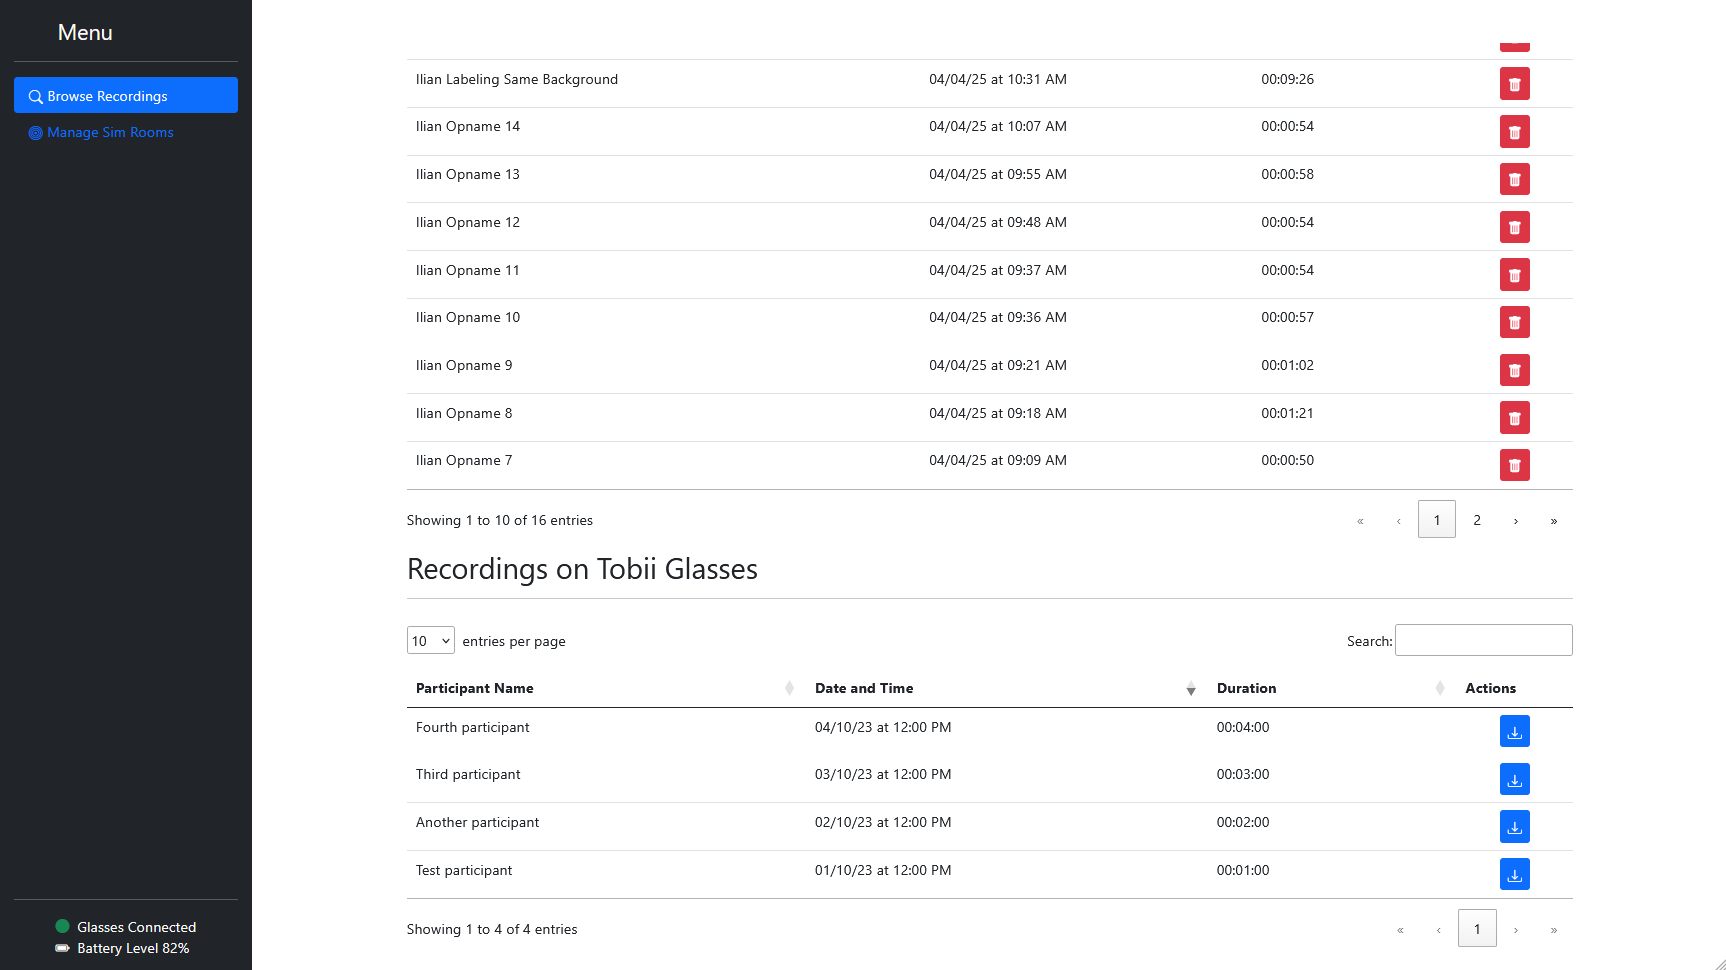
\includegraphics[width=1\textwidth]{browse-recordings-connected.png}
  \caption[]{\label{fig:browse-recordings-connected} Bij dit voorbeeld is de bril wel verbonden met de computer. Men ziet linksonder de batterlijstatus van de bril. In de onderste tabel is het mogelijk om opnames te importeren vanuit de bril naar de computer. }
\end{figure}

\subsubsection{Simulatieruimten en Objecten}

Eens de opnames zijn geïmporteerd, kunnen we overgaan tot het definiëren van de objecten in de kalibratie-opnames. Één van de design-keuzes was om met zogenaamde `simulatieruimten` te werken die verschillende omgevingen voorstellen, elk met hun eigen objecten.
Men kan zich dus voorstellen dat men niet enkel in het Zorglab werkt, maar bijvoorbeeld ook in een echt ziekenhuis of een woonzorgcentrum. Het doel was dus om de applicatie zo gebruiksvriendelijk mogelijk te maken, om het werk van de trainers te vergemakkelijken.

\begin{figure}[H]
  \centering
  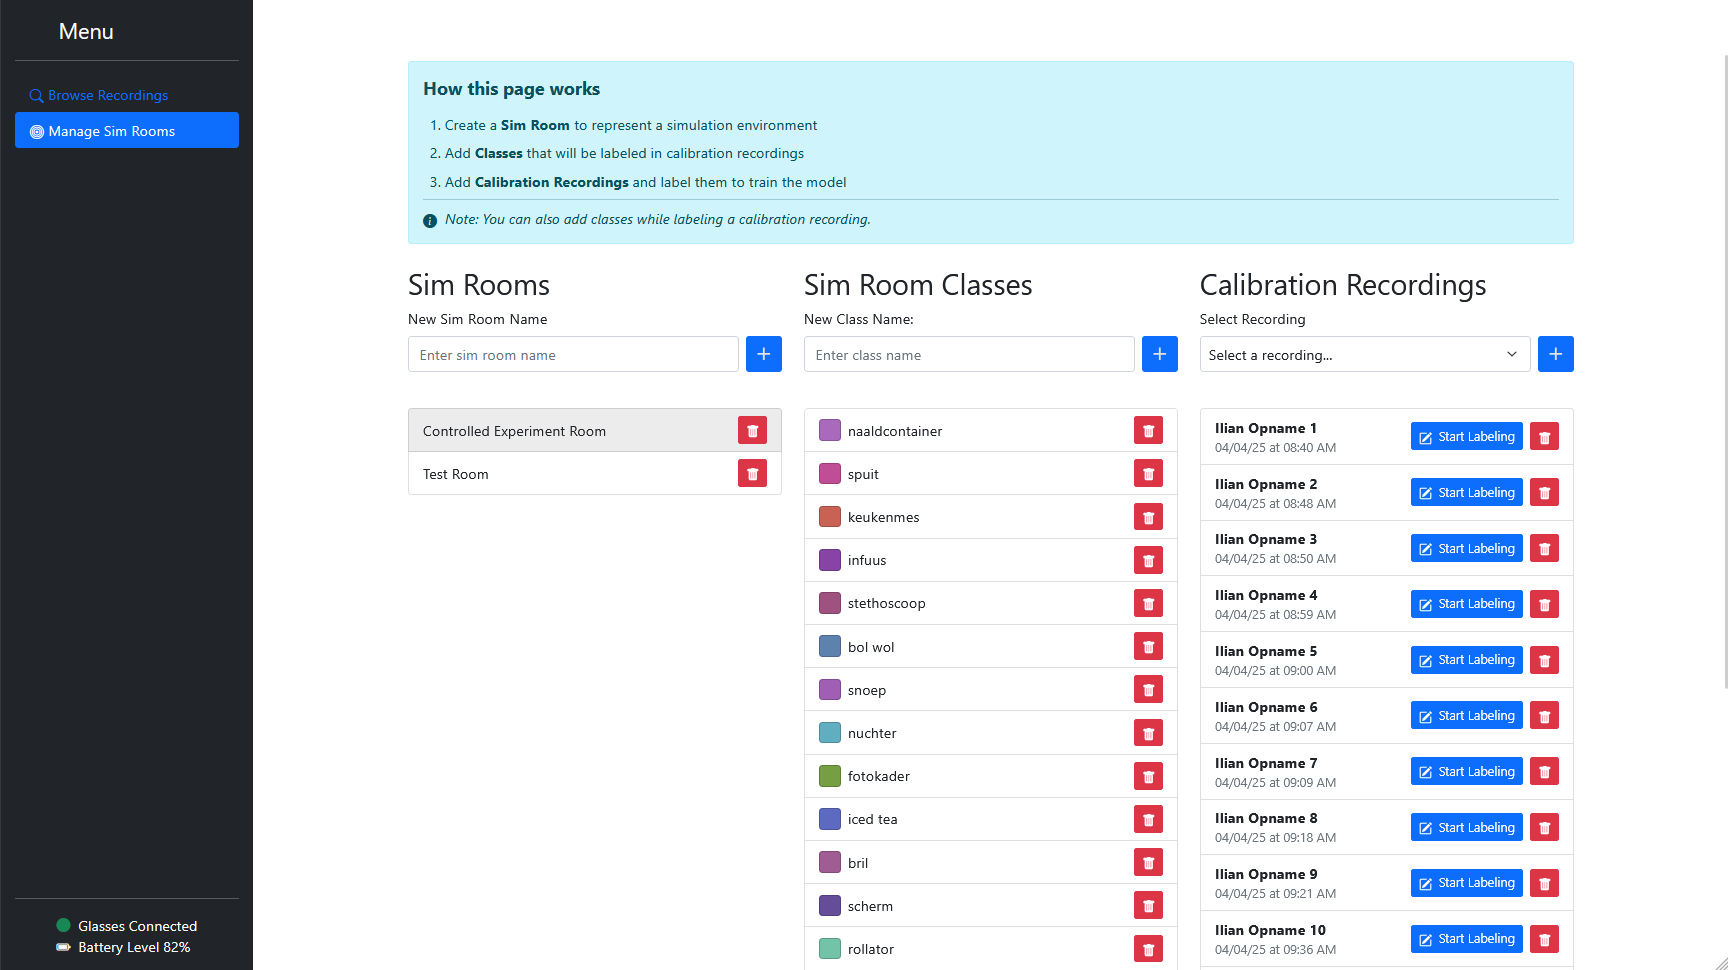
\includegraphics[width=1\textwidth]{simrooms.png}
  \caption[]{\label{fig:simrooms} Voorbeeld van de `Manage Sim Rooms'-pagina waar de simulatieomgevingen kunnen worden gedefinieerd. Hier is de `Controlled Experiment Room' geselecteerd, met een aantal objecten en kalibratie-opnames. }
\end{figure}

In figuur \ref{fig:simrooms} is een voorbeeld te zien van de pagina waar simulatieomgevingen kunnen worden gedefinieerd. 
Deze pagina heeft drie kolommen:
\begin{itemize}
    \item De eerste kolom toont de reeds gedefinieërde simulatieomgevingen, met hun naam, een knop om deze te verwijderen, en een invoerveld om meer simulatieomgevingen toe te voegen.
    \item Wanneer een simulatieomgeving is geselecteerd, worden de bijbehorende objecten getoond in de tweede kolom. Elk object krijgt automatisch een kleur toegewezen die ook gebruikt zal worden in de labeling-tool, en eventueel de visualisatie van de metrieken.
    \item In de derde kolom kan men geïmporteerde opnames selecteren om deze te gebruiken als kalibratie-opnames. Elke kalibratie-opname heeft een knop "Start Labeling". Wanneer men hierop klikt, wordt de labeling-tool geopend met de geselecteerde opname.
\end{itemize}

Merk op dat het mogelijk is om welke opname dan ook te selecteren als kalibratie-opname, waardoor ook praktijkopnames kunnen worden gebruikt!
Zo kunnen we reeds gemaakte opnames van studenten ook gebruiken om de analysemodellen te trainen.
Dit stelt de applicatie eventueel in staat om de opnames te analyseren op basis van manuele annotaties van de trainers.
Deze aanpak zal meer tijd vergen, maar is veel nauwkeuriger dan een automatische analyse. Aangezien het in deze bachelorproef gaat om geautomatiseerde analyse, werd deze optie niet verder uitgewerkt.

Wanneer men een kalibratie-opname verwijdert, heeft dit geen invloed op de opname zelf, maar enkel op de associatie met de simulatieomgeving.
Indien er met de opname werd gelabeld binnen deze simulatieomgeving, worden deze annotaties wel verwijderd. 
Hetzelfde geldt voor de objecten: indien een object wordt verwijderd, worden ook de annotaties die gemaakt werden met dit object in alle kalibratie-opnames verwijderd.

\subsubsection{Labeling Tool}

We hebben het al eerder gehad over de labeling-tool, maar hoe werkt deze nu precies? Dit is één van de belangrijkste onderdelen van de applicatie, en ook het meest complexe.
De labeler kunnen we openen door op de knop "Start Labeling" te klikken van een kalibratie-opname binnen de `Manage Sim Rooms'-pagina.
In de achtergrond worden alle individuele frames uit de opname gehaald en in een map opgeslagen, waardoor het enige tijd kan duren voor de tool opent. De specifieke implementatieredenen hiervoor komen later aan bod.
Het doel van de labeler is om een masker (en een `bounding box') te verkrijgen binnen elke frame van de opname waarin een object zich bevindt.
Natuurlijk zou dit een grote tijdsinvestering vragen bij een volledig manuele tool: Aangezien de framerate van de eyetracker 25FPS is, zou dit betekenen dat we 1500 frames moeten labelen voor een opname van 1 minuut, en dit voor elk object dat we willen labelen.
Het probleem werd opgelost met een semi-automatische labelingtool. Daarbij hoeft men enkel in minder dan tien frames per object te klikken. De tool volgt vervolgens elk object automatisch doorheen de hele opname.
De functies van de labeling-tool worden hieronder verder toegelicht.

\begin{figure}[H]
  \centering
  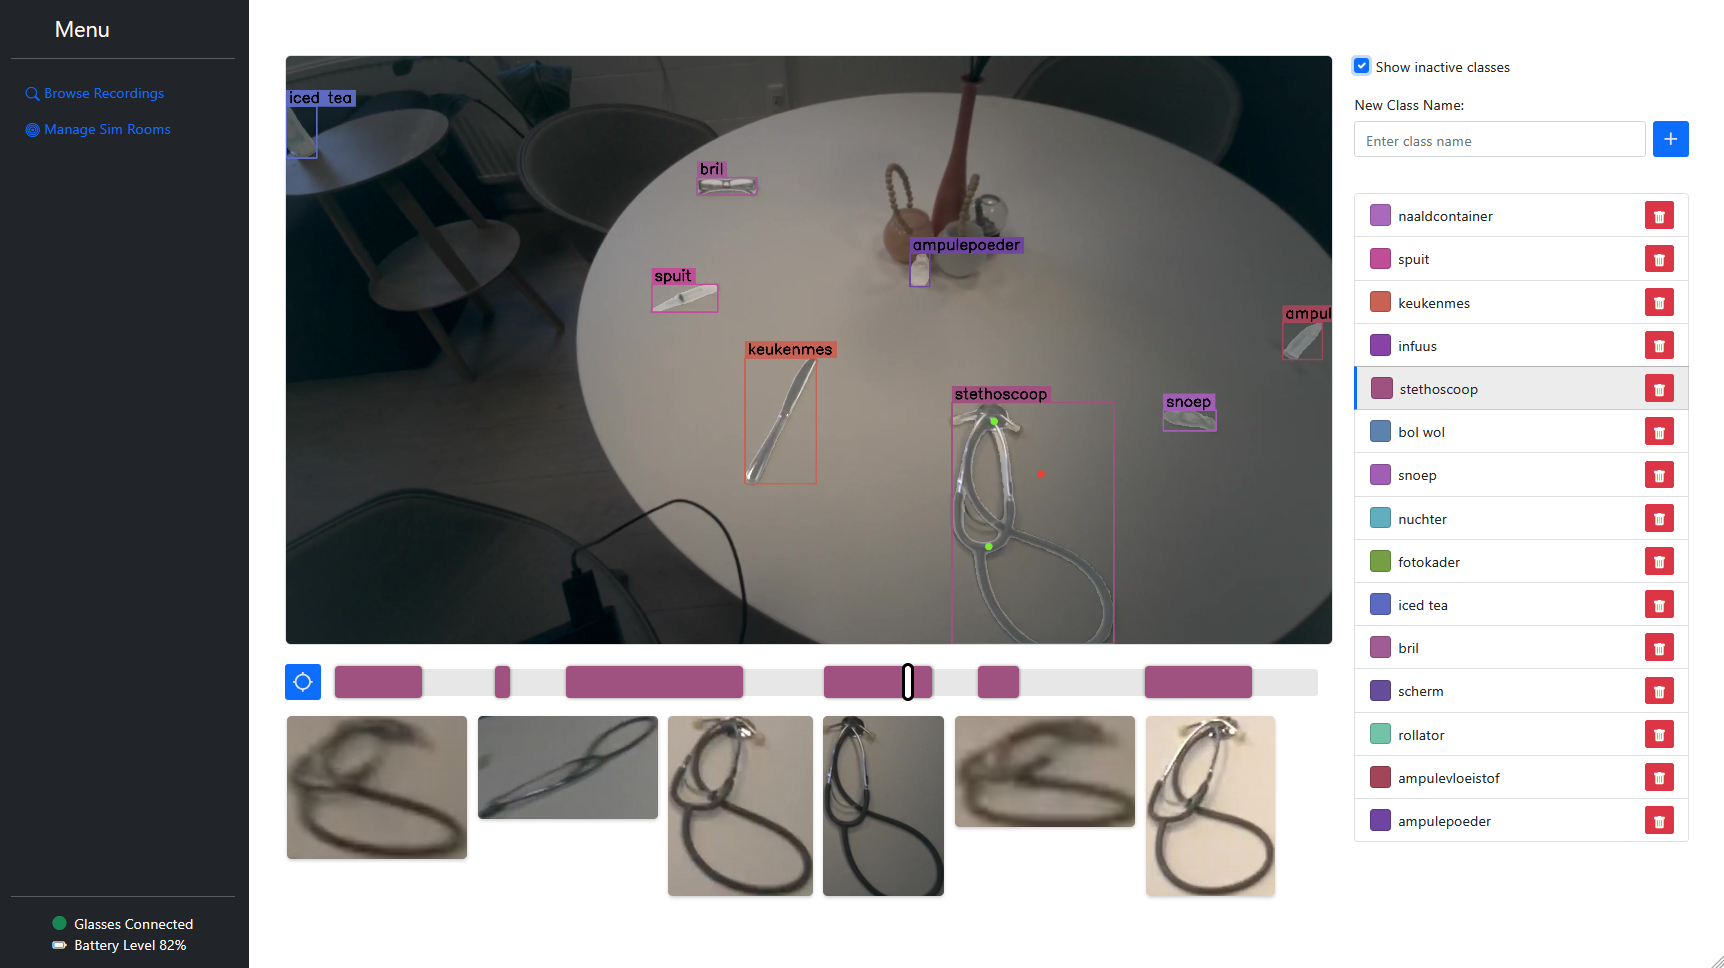
\includegraphics[width=1\textwidth]{labeler.png}
  \caption[]{\label{fig:labeler} Een screenshot van de labeling-tool met vier onderdelen: de labeling-canvas, de tijdlijn, de objectenlijst rechts, en een lijst van gemaakte annotaties onderaan. In dit voorbeeld is het object `Stethoscoop' geselecteerd. }
\end{figure}

Eenmaal de labeling-tool geopend is, zien we een pagina met vier onderdelen (zie figuur \ref{fig:labeler}).
Linksboven zien we het `labeling-canvas', waar de huidige geselecteerde frame van de opname wordt getoond. Onder het canvas is er een tijdlijn die aangeeft waar we ons bevinden in de opname. De tijdlijn markeert ook welke frames het gevolgde object bevatten. 
Binnen deze canvas kunnen we objecten labelen door eerst een object in de lijst rechts te selecteren, en vervolgens te klikken op het canvas.
Hierbij kunnen we een linkermuisklik gebruiken om aan te geven welke delen van de afbeelding deel uitmaken van het object dat we willen labelen (zie de stethoscoop in figuur \ref{fig:labeler}). Met de rechtermuisklik geven we aan welke regio's buiten het object vallen.
Deze zijn respectievelijk gemarkeerd met een groene en een rode stip. Als we met de muis over een stip gaan, wordt deze gemarkeerd. Vervolgens kunnen we erop klikken om de stip te verwijderen.
Na elke muisklik worden het masker en de bijbehorende \textit{bounding box} automatisch geüpdatet om feedback te geven aan de gebruiker.
Onder de tijdlijn zien we een reeks annotaties die we hebben gemaakt, van links naar rechts gesorteerd op tijd. Men kan op deze annotaties klikken om naar de bijbehorende frame te gaan, en ze ook verwijderen door met de muis erover te gaan en op de rode knop te klikken.
Indien men alle stippen verwijdert, wordt de annotatie ook verwijderd.
Eens we tevreden zijn met de annotaties, kunnen we op de blauwe `tracking'-knop klikken aan de linkerkant van de tijdlijn.
Dit start de automatische tracking van het huidige geselecteerde object doorheen de opname, zoals getoond in figuur \ref{fig:labeler-tracking}. 

\begin{figure}[H]
  \centering
  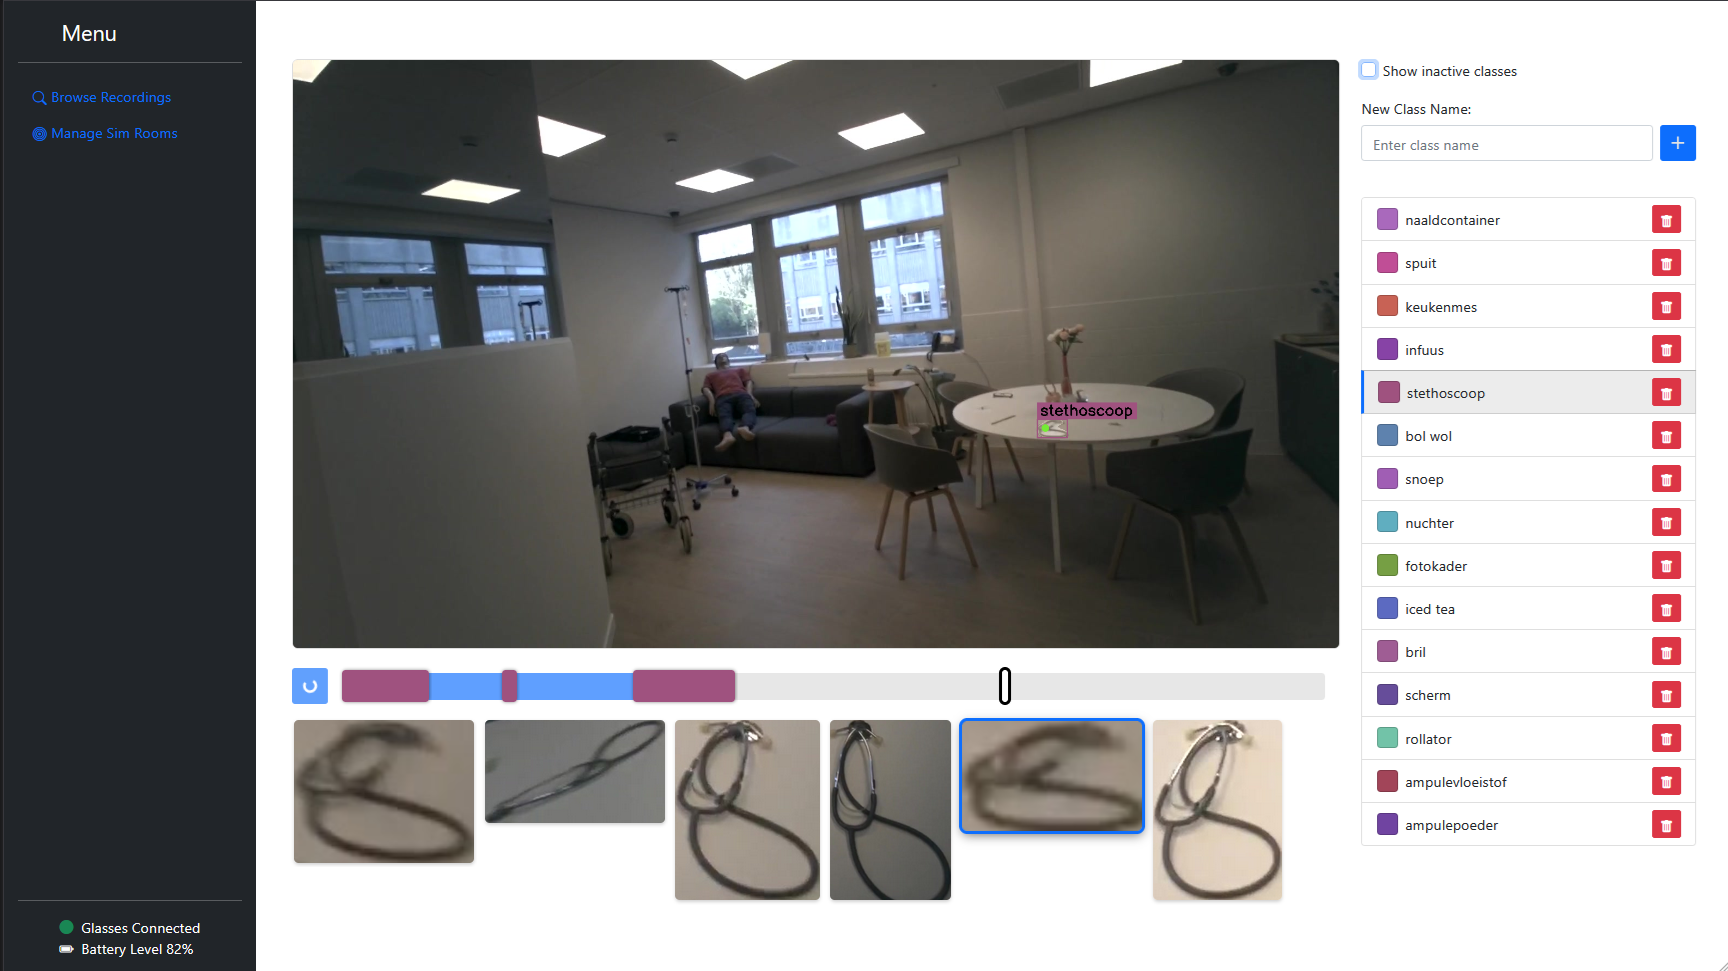
\includegraphics[width=1\textwidth]{labeler-tracking.png}
  \caption[]{\label{fig:labeler-tracking} In deze screenshot zien we dat er een tracking-opdracht gaande is. Hier is ook de optie `Show inactive classes' uitgevinkt, waardoor enkel het actieve object wordt getoond. }
\end{figure}

Om prestatieredenen zullen niet alle frames bekeken worden binnen deze tracking-opdracht. Een annotatie wordt als basis gebruikt voor tracking, en wanneer het object voor een bepaalde tijd uit het beeld verdwijnt, wordt de trackingopdracht stopgezet tenzij er nog annotaties overblijven.
Over het algemeen hebben we slechts één annotatie nodig voor elk gedeelte van de video waarin het object voortdurend in beeld is. Soms zijn echter meerdere annotaties per gedeelte nodig om het trackingresultaat te optimaliseren.
Het specifieke algoritme dat bedacht werd voor de tracking komt aan bod in de technische sectie van dit onderdeel.
Tenslotte bestaat de mogelijkheid dat er veel objecten in beeld zijn waardoor maskers, bounding boxes en labels elkaar overlappen. Om deze reden kunnen we rechtsboven een optie `Show inactive classes', uitvinken om enkel het actieve object te tonen in het canvas.

\subsubsection{Analyse van Eyetracking-Opnames}

Hoewel het aanvankelijk de bedoeling was, werd in de context van deze bachelorproef, geen werkende analyse-tool ontwikkeld maar enkel een proof-of-concept.
De labeling-tool was in dit opzicht de belangrijkste component, omdat deze de annotaties genereert die nodig zijn voor de analyse.
Aangezien de resultaten van de analyses niet betrouwbaar waren, werd hier ook geen pagina voor ontwikkeld.
Indien men in de toekomst een betrouwbaar analysemodel kan ontwikkelen, bestaat de mogelijkheid om een nieuwe pagina te maken die de resultaten van de analyses toont.
Naast de pagina dient dan ook een bijbehorende optie in de navigatiekolom aangemaakt te worden.
De analyses die uitgevoerd werden in deze bachelorproef komen aan bod in Hoofdstuk~\ref{ch:experiment}.

\section{Technische Specificaties}

Voor de ontwikkeling van de applicatie werd een lichtgewicht, modulaire softwarestack gekozen, afgestemd op de specifieke noden van het project.
Er is geopteerd voor een web-applicatie die lokaal kan draaien op een laptop (met een degelijke GPU) of een desktop computer, en die via een browser toegankelijk is.

\begin{itemize}
    \item \textbf{Backend Framework:} Python met \texttt{FastAPI} werd gekozen omwille van zijn hoge prestaties, asynchrone mogelijkheden (belangrijk voor I/O-intensieve taken zoals data-import en analyse), automatische documentatie en type hinting-integratie.
    \item \textbf{Frontend Aanpak:} In plaats van een zwaar JavaScript-framework, werd geopteerd voor \texttt{HTMX}. Dit laat toe om dynamische interacties te bouwen door HTML direct uit te wisselen met de server, wat de complexiteit van de frontend aanzienlijk reduceert. \texttt{Jinja2} dient als templating engine om deze HTML server-side te genereren. Tenslotte werd \texttt{Bootstrap} gebruikt voor de opmaak van de applicatie.
    \item \textbf{Database:} Een \texttt{SQLite} database werd gebruikt vanwege de eenvoud en het feit dat de applicatie bedoeld is voor lokaal gebruik, waardoor een complexe database server overbodig is. \texttt{SQLAlchemy} werd ingezet als ORM (Object-Relational Mapping) voor een gestructureerde interactie met de database vanuit Python.
    \item \textbf{Hardware Communicatie:} Voor de interactie met de Tobii Pro Glasses 3 werd de officiële \texttt{g3pylib} SDK gebruikt, die toegang biedt tot opnames en statusinformatie via de WiFi-verbinding.
    \item \textbf{Development \& Kwaliteitsborging:} \texttt{Poetry} werd gebruikt voor dependency management. Strikte type hinting met \texttt{Mypy} en code linting/formatting met \texttt{Ruff} dragen bij aan de robuustheid en onderhoudbaarheid van de code. \texttt{Docker} werd ingezet om de applicatie te containeriseren, wat zorgt voor een consistente uitvoeringsomgeving en eenvoudige deployment.
\end{itemize}
Deze keuzes resulteerden in een applicatie die relatief eenvoudig te onderhouden en verder te ontwikkelen is, conform de doelstelling om iteratieve verbeteringen in volgende bachelorproeven mogelijk te maken.

\subsection{Softwarearchitectuur}

De applicatie volgt een gelaagde architectuur om een duidelijke scheiding van verantwoordelijkheden (Separation of Concerns) te waarborgen en de onderhoudbaarheid en testbaarheid te verhogen. 
De data en requests vloeien doorgaans van de \texttt{frontend} via de \texttt{routes} naar de \texttt{services}, die vervolgens de \texttt{repositories} aanroepen voor databasetoegang (zie figuur \ref{fig:software-architectuur}).

\begin{figure}[H]
  \centering
  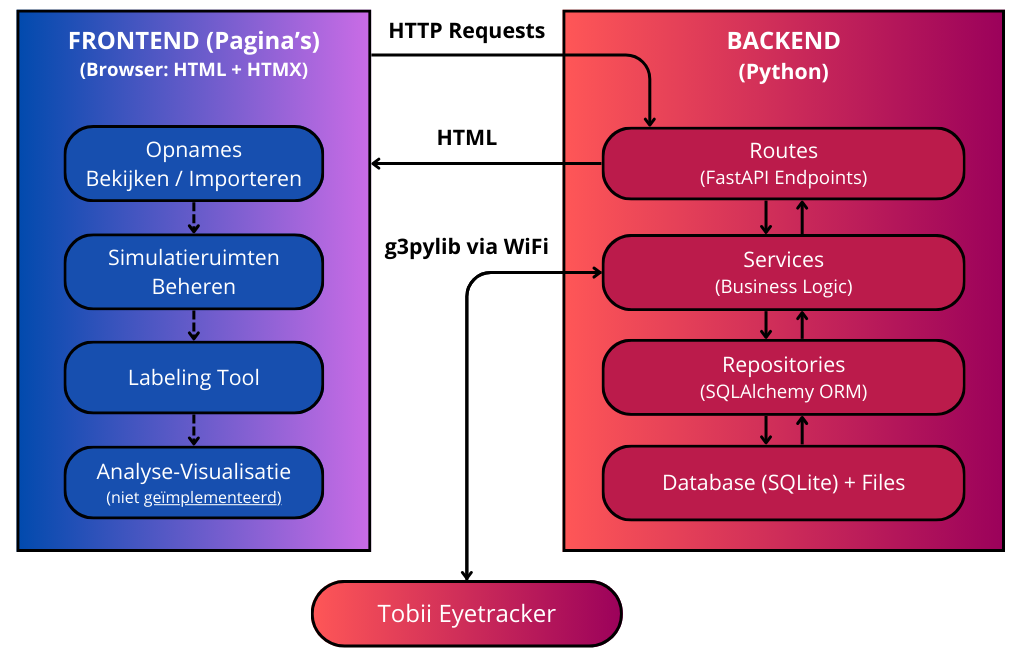
\includegraphics[width=0.8\textwidth]{software-architectuur.png}
  \caption[]{\label{fig:software-architectuur} Software-architectuur van de applicatie. De applicatie is opgebouwd uit verschillende lagen die elk hun eigen verantwoordelijkheden hebben. }
\end{figure}
% Link naar canva: https://www.canva.com/design/DAGmr8n_Umg/6k1gqiCpq2hON75Jq9H17Q/edit?utm_content=DAGmr8n_Umg&utm_campaign=designshare&utm_medium=link2&utm_source=sharebutton

\subsubsection{Frontend (HTML, HTMX, en Jinja2)}

De gebruikersinterface (UI) wordt weergegeven in de browser en is opgebouwd uit HTML-pagina's die server-side worden gegenereerd met behulp van de \texttt{Jinja2} templating engine.
Deze engine maakt het mogelijk om inhoud (data vanuit de Backend) te integreren in de HTML-pagina's door gebruik te maken van variabelen en controle-structuren.
Voor de dynamische aspecten van de applicatie, waaronder het bijwerken van de UI zonder de volledige pagina te herladen, wordt \texttt{HTMX} ingezet.

\texttt{HTMX} maakt het mogelijk om via HTML-attributen aanroepen te doen naar de backend (vb: als een knop wordt ingedrukt).
De backend genereert vervolgens het gevraagde HTML-fragment---zoals een tabel met opnames of een lijst van objecten---die HTMX vervolgens injecteert in de huidige pagina.
Op deze manier kunnen eenvoudige interacties worden gerealiseerd zonder de noodzaak van een volledig JavaScript-framework zoals React of Vue.js.

Binnen de `Browse Recordings'-en `Manage Sim Rooms'-pagina's is HTMX grotendeels voldoende, maar toch valt JavaScript niet volledig te vermijden.
De labeling-tool vergt immers complexe interacties die niet eenvoudig gerealiseerd kunnen worden met enkel HTML en HTMX.
Zo werd de labeling-tool opgesplitst in vijf componenten die elk hun eigen verantwoordelijkheden hebben:
\begin{itemize}
    \item De \texttt{labeling-canvas} die de huidige frame toont en het mogelijk maakt om objecten te labelen.
    \item De \texttt{tijdlijn} die de voortgang van de opname toont en het mogelijk maakt om naar een specifieke frame te navigeren.
    \item De \texttt{objectenlijst} die de beschikbare objecten toont en het mogelijk maakt om objecten te beheren en te selecteren.
    \item De \texttt{annotatielijst} die de gemaakte annotaties van het momenteel geselecteerde object toont.
    \item De \texttt{labeling settings} die instellingen van de labeling-tool toont (`Show inactive classes').
\end{itemize}
Elk van deze componenten communiceert apart via HTMX-attributen met de backend, en kunnen onafhankelijk van elkaar worden geladen.
Wanneer toch communicatie nodig is tussen de componenten, gebeurt dit via \texttt{Events} die door de componenten worden uitgezonden en opgevangen.
Een voorbeeld hiervan is wanneer de gebruiker klikt op de tijdlijn om naar een specifieke frame te navigeren.
De tijdlijn stuurt een event naar de labeling-canvas, die vervolgens een aanroep doet naar de backend om de juiste frame op te halen.

Aangezien het gaat om een single-user applicatie, is het toch mogelijk om een groot deel van de logica over te dragen aan de backend.
De frontend is dus voornamelijk verantwoordelijk voor de presentatie van de data en de interactie met de gebruiker.
De backend is verantwoordelijk voor de verwerking van de data, en het bijhouden van de status van de applicatie (de huidige frame, de geselecteerde objecten, de machine-learning modellen, etc.).

\subsubsection{Backend (Python met FastAPI)}

De backend, geschreven in Python met het \texttt{FastAPI} framework, is verantwoordelijk voor het verwerken van requests, 
het uitvoeren van de businesslogica, en de interactie met de datalaag en externe hardware.

\paragraph{Routes (FastAPI Endpoints)}
De \texttt{routes} definiëren de API-endpoints waarnaar de frontend requests stuurt.
Deze laag ontvangt HTTP-requests, valideert inkomende data 
(via Pydantic modellen die FastAPI automatisch uit request bodies of query parameters haalt), 
roept de juiste methoden aan in de \texttt{services}-laag, en formatteert de respons. 
Voor HTMX-requests is dit typisch een HTML-fragment gerenderd met Jinja2; voor andere endpoints kan dit JSON zijn 
(bv. het ophalen van annotatiepunten voor de labeler).

\paragraph{Services (Business Logic)}
De \texttt{services}-laag bevat de kernlogica van de applicatie.
Services coördineren operaties en implementeren de business rules. 
Ze zijn ontkoppeld van de HTTP-laag en de directe database-implementatie. 
In plaats daarvan gebruiken ze methoden uit de \texttt{repositories}-laag voor datatoegang en -persistentie, 
en kunnen ze andere utilities of externe bibliotheken aanroepen (bv. \texttt{g3pylib} voor communicatie met de Tobii-bril, of \texttt{SAM2ImagePredictor} voor segmentatie).

\paragraph{Repositories (Data Access)}
De \texttt{repositories}-laag vormt de abstractielaag boven de database en het filesysteem.
Het bevat alle logica voor het ophalen, opslaan, en beheren van data in de \texttt{SQLite} database via \texttt{SQLAlchemy} ORM.
Ook bevat het logica voor het beheren van bestanden op de schijf, zoals resultaten van de labeling-tool of de video-opnames.
Dit zorgt ervoor dat de \texttt{services}-laag onafhankelijk is van de specifieke database-implementatie.

\subsection{Database}

We hebben het al eerder gehad over opnames, simulatieomgevingen, objecten en annotaties, maar hoe worden deze nu opgeslagen in de database?
Om een beter zicht te krijgen op de database, werd er een Entity-Relationship Diagram (ERD) gemaakt dat de verschillende entiteiten en hun onderlinge relaties toont (zie figuur \ref{fig:erd}).

\begin{figure}[H]
  \centering
  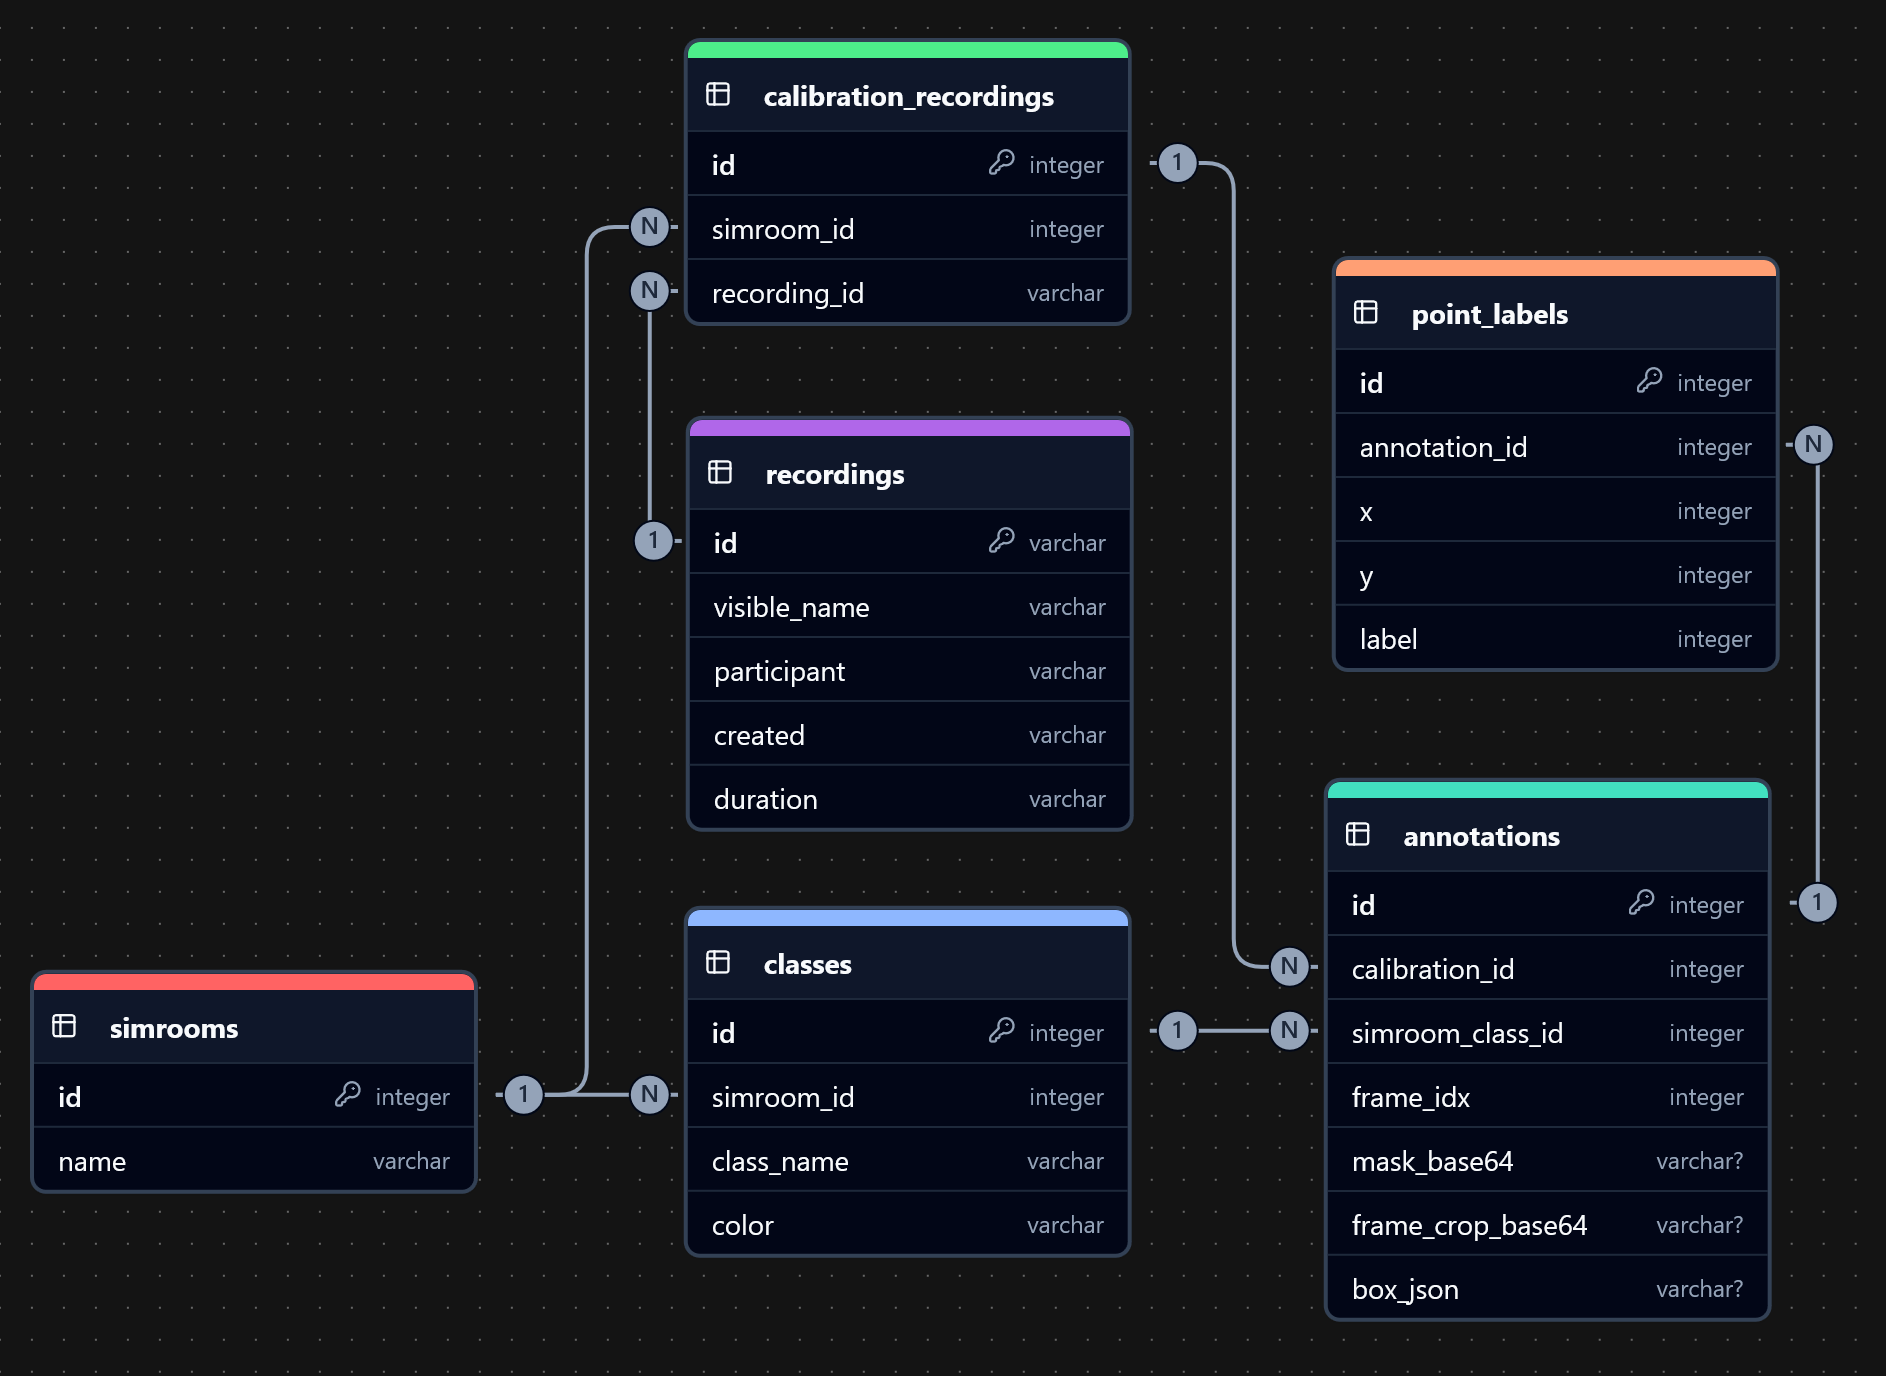
\includegraphics[width=0.8\textwidth]{erd.png}
  \caption[]{\label{fig:erd} Entity-Relationship Diagram (ERD) van de applicatie. De verschillende entiteiten en hun onderlinge relaties worden weergegeven: simulatieruimten, objecten (classes), opnames, kalibratie-opnames, annotaties, en point-labels. }
\end{figure}

\begin{itemize}
  \item \textbf{simrooms} zijn de verschillende omgevingen waarin de opnames worden gemaakt. 
  Elke simulatieomgeving heeft een naam en kan meerdere objecten bevatten.
  \item \textbf{classes} zijn de verschillende objecten die in de simulatieomgeving aanwezig zijn. 
  Elk object heeft een naam, een kleur, en kan meerdere annotaties bevatten.
  \item \textbf{recordings} zijn de video-opnames die gemaakt worden met de eyetracker. 
  Elke opname heeft een naam, een datum, en een duur. 
  Een opname kan ook dienen als kalibratie-opname voor meerdere simulatieruimten. 
  Opnames hebben ook een pad naar hun video-bestand en hun blik-data bestand. 
  Deze paden worden niet opgeslagen in de database, maar worden gegenereerd op basis van het \texttt{id} van de opname. 
  \item \textbf{calibration\_recordings} zijn louter een referentie naar de opname die als kalibratie-opname wordt gebruikt 
  voor de simulatieomgeving. Ze kunnen meerdere annotaties bevatten.
  \item \textbf{annotations} worden gemaakt in de labeling-tool en hebben een \texttt{class}, een \texttt{frame index}, 
  een base64-gecodeerde afbeelding van het masker en van de regio in de originele frame, en een bounding box. Zowel het base64-gecodeerde 
  masker en de bounding-box worden getoond in de labeler bovenop de originele frame. De bounding-box is de rechthoek die de regio van de 
  annotatie omsluit, met het json formaat: \texttt{[x1, y1, x2, y2]}. Hier zijn \texttt{x1} en \texttt{y1} de coördinaten van de 
  linkerbovenhoek van de rechthoek, en \texttt{x2} en \texttt{y2} de coördinaten van de rechteronderhoek. 
  Tenslotte wordt ook een `crop' van de originele frame opgeslagen, dat enkel de regio van de annotatie bevat. 
  Dit is een afbeelding van dezelfde grootte als het masker, en wordt gebruikt om de annotatie te tonen in de annotatielijst onderaan de labeler.
  \item \textbf{point\_labels} zijn de individuele punten die aan een annotatie worden gegeven. Elk point-label heeft een x- en y-coördinaat, en een label dat aangeeft of het punt binnen (1) of buiten (0) de annotatie ligt.
\end{itemize}

Merk op dat de geautomatiseerde tracking-resultaten niet in de database worden opgeslagen, maar enkel de manuele annotaties.
Dit is omdat tracking grote hoeveelheden data generereert die op een optimale manier moeten worden opgeslagen.
De tracking-resultaten worden opgeslagen in een aparte map, onderverdeeld per kalibratie-opname en per klasse.
Elke file bevat de tracking-resultaten van één object in één kalibratie-opname, met als naam de frame index.
Ze worden opgeslagen in \texttt{.npz}-bestanden, die een gecomprimeerd formaat zijn voor numpy arrays.
Ze bevatten de volgende data:
\begin{itemize}
  \item \texttt{mask}: de gecomprimeerde versie van het masker dat werd gegenereerd door het segmentatie-algoritme.
  \item \texttt{bbox}: \texttt{[x1, y1, x2, y2]} de coördinaten van de bounding-box die het object omsluit.
  \item \texttt{roi}: de regio van de originele frame die overeenkomt met het masker.
  \item \texttt{class\_id}: de id van de klasse waartoe het object behoort. 
  Zo kan andere informatie over het object---zoals de naam en de kleur---worden opgehaald uit de database.
  \item \texttt{frame\_index}: de index van de frame waarin het object werd getracked.
\end{itemize}

Deze tracking-resultaten zullen uiteindelijk als basis dienen voor de analyses die uitgevoerd worden op de eyetracking-opnames van de studenten.
Hoe worden deze resultaten nu precies gegenereerd vanuit de manuele annotaties? Dit zullen we verder bekijken in de volgende sectie.


\chapter{Experimenteel Onderzoek}
\label{ch:experiment}

In het voorgaande hoofdstuk werd de ontwikkeling van de proof-of-concept softwareapplicatie uitvoerig besproken.
Voor ontwikkelingsdoeleinden werd gebruik gemaakt van een dataset die thuis werd opgenomen met de Tobii Pro Glasses 3.
Deze dataset was echter niet geschikt voor evaluatie van de uiteindelijke analysemethoden, aangezien ze door de onderzoeker zelf werden opgenomen en geen objecten bevatten die relevant zijn voor de zorgcontext.
Om een dataset te verkrijgen die wel aan deze kwaliteitseisen voldoet, werd er een experiment opgezet in het Zorglab van HoGent waarin studenten gevraagd om de eyetracker te dragen en te kijken naar verschillende objecten.
De opzet, uitvoering en de resulterende data van dit experiment worden in dit hoofdstuk nader toegelicht.

\section{Doelstellingen van het Experiment}

Het hoofddoel van het experiment was om een dataset te creëren die als grondwaarheid kon dienen voor het valideren van de twee kernmetrieken van de PoC applicatie:
\begin{itemize}
    \item De objecten die de studenten hebben bekeken.
    \item De tijdsduur dat de studenten naar deze objecten hebben gekeken.
\end{itemize}
Om deze validatie mogelijk te maken, werden twee soorten opnames gegenereerd. 
Ten eerste werden er zogenaamde \textit{kalibratieopnames} gemaakt door de onderzoeker zelf. 
Deze dienden primair om de computervisiemodellen binnen de analyses te initialiseren met de visuele kenmerken van de te detecteren objecten. 
Ten tweede werden er \textit{evaluatieopnames} verzameld waarbij studenten de eyetracker droegen en de observatietaak uitvoerden. 
Deze laatste categorie vormt de kern van de te analyseren data waarvoor de ground-truth werd vastgesteld.

Naast het genereren van deze ground-truth, had het experiment ook als doel om de robuustheid van de ontwikkelde analysemethoden te onderzoeken. 
Dit omvatte het evalueren van de prestaties van het systeem onder invloed van verschillende factoren, waaronder:
\begin{itemize}
    \item De invloed van \textbf{variërende kijkafstanden tot objecten} op de detectieaccuraatheid, resulterend in variaties in objectgrootte en detail in het camerabeeld.
    \item De prestaties van de modellen bij \textbf{diverse objectkarakteristieken}, zoals verschillen in vorm, grootte, textuur en mate van transparantie.
    \item De impact van \textbf{wisselende achtergronden} op de betrouwbaarheid van de objectherkenning.
\end{itemize}

\section{Opzet van het Experiment}

De concrete uitwerking van het experiment omvatte de inrichting van de experimentele omgeving, de keuze van kritische objecten, het opstellen van een gestandaardiseerde procedure, en de selectie van deelnemers.

\subsection{Experimentele Omgeving en Materialen}

De experimentele opnames vonden plaats in het Zorglab van HOGENT, dat beschikt over verschillende gesimuleerde zorgomgevingen. 
Voor deze bachelorproef werd specifiek gebruik gemaakt van de ruimte die is ingericht als een \textbf{woonkameromgeving}. 
Deze setting omvat typische elementen zoals een zithoek met een zetel, een keukengedeelte en een eettafel. 
Hoewel het Zorglab ook een gesimuleerde ziekenhuiskamer met twee bedden ter beschikking stelt, werd omwille van praktische overwegingen, 
zoals de positionering van objecten en de bewegingsvrijheid voor de deelnemers, gekozen voor de woonkameropstelling.

\begin{figure}[H]
  \centering
  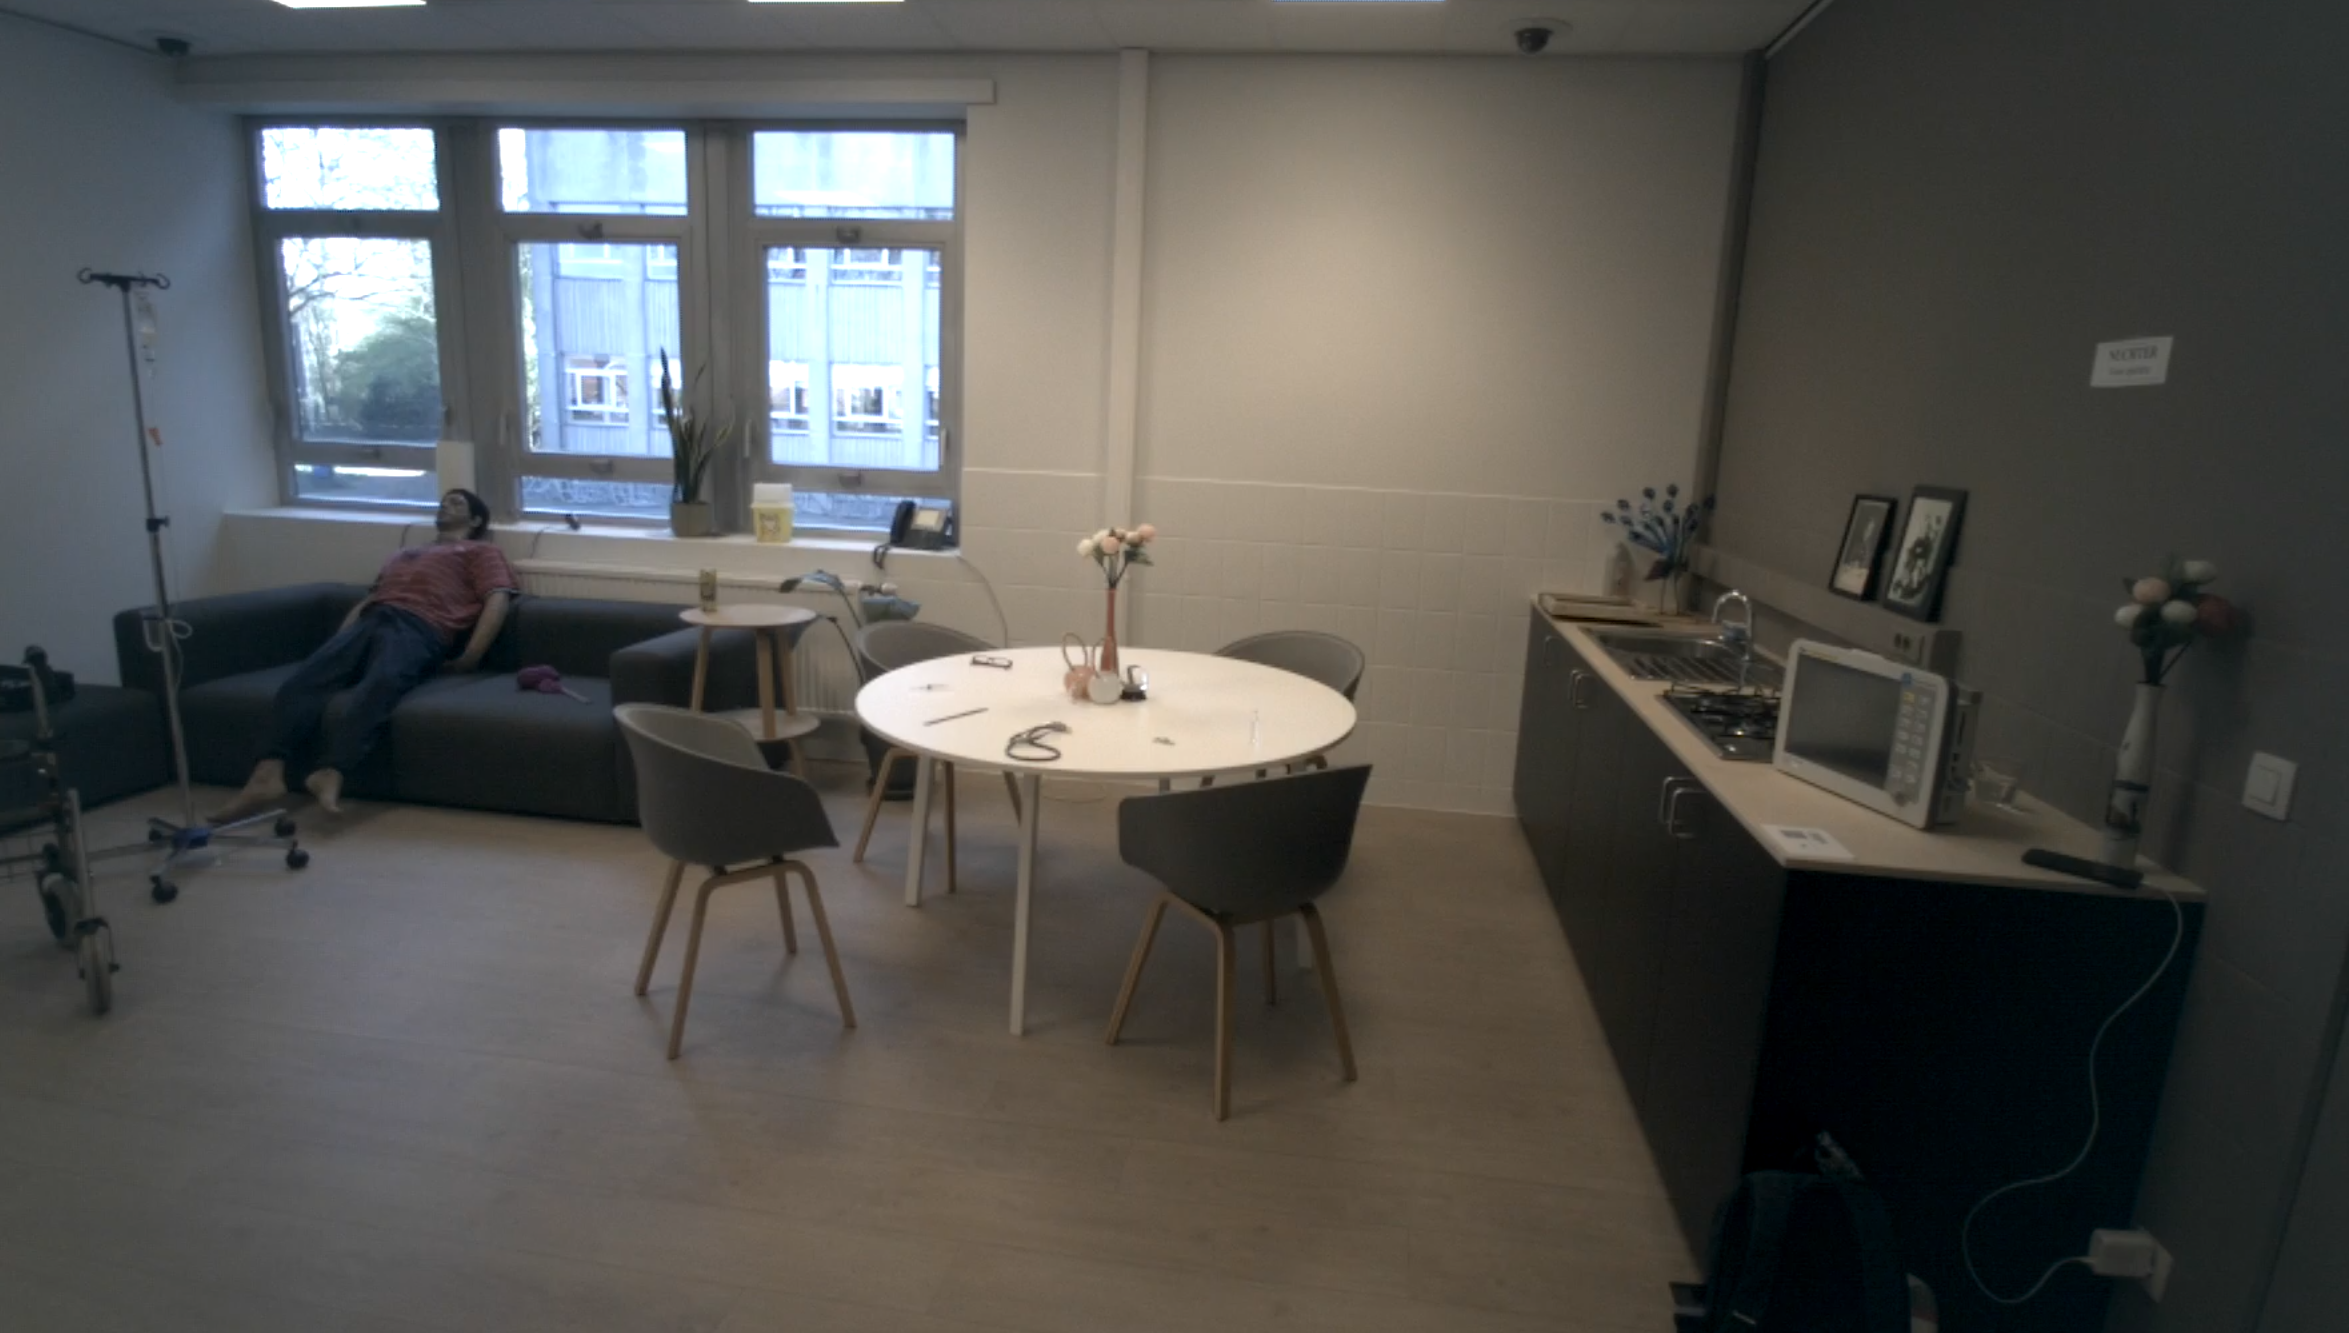
\includegraphics[width=1\textwidth]{zorglab.png}
  \caption[]{\label{fig:zorglab} De woonkameromgeving in het Zorglab van HoGent.}
\end{figure}

Het Zorglab beschikt over een uitgebreid assortiment aan objecten die ingezet kunnen worden tijdens simulatietrainingen. 
Uit deze collectie werden voor 15 specifieke objecten geselecteerd (zie Figuur~\ref{fig:object_grid}).
Dit aantal werd gekozen als een pragmatisch compromis tussen het verkrijgen van voldoende variatie in objecttypes 
die relevant zijn voor de zorgcontext en de technische uitdagingen, en het behouden van een haalbare werklast voor de latere annotatie van de grondwaarheid.
Deze objecten werden vervolgens in de woonkameromgeving geplaatst.

\begin{figure}[H]
  \centering
  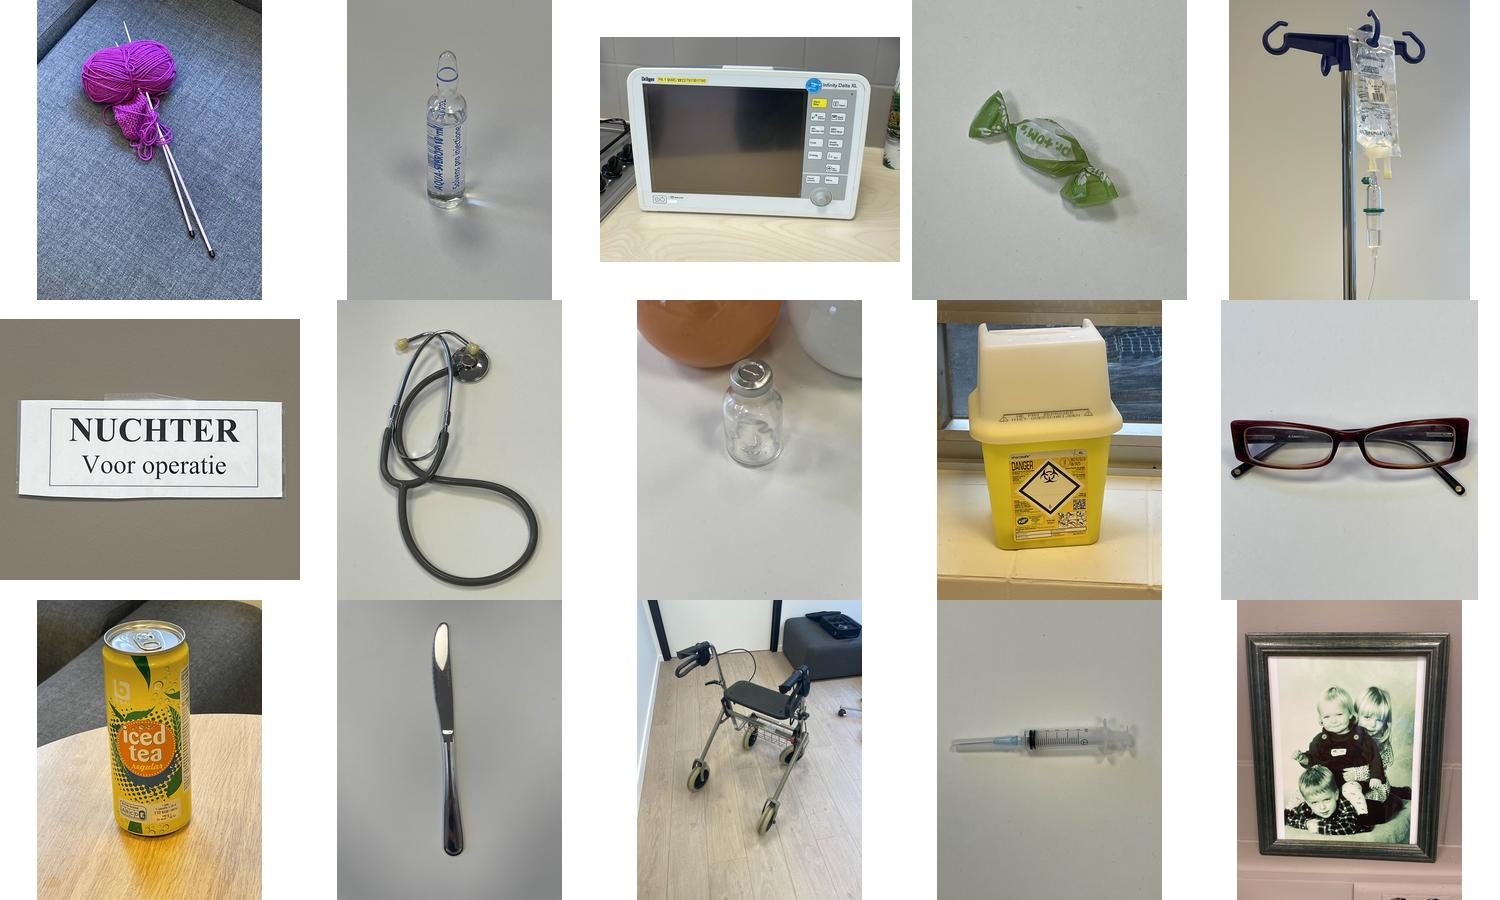
\includegraphics[width=0.8\textwidth]{object_grid.jpg}
  \caption[]{\label{fig:object_grid} De geselecteerde objecten voor het experiment. Van links naar rechts en van boven naar beneden: 
  een bol wol, een ampule met vloeistof, een monitor, een snoepje, een infuus, een indicator "Nuchter voor operatie", een stethoscoop, een transparante ampule, een naaldcontainer, een bril, een blikje iced tea, een keukenmes, een rollator, een spuit, een fotokder. 
  }
\end{figure}

Elk van deze objecten werd geselecteerd om redenen die zowel te maken hebben met de zorgcontext als met de technische haalbaarheid van de detectie:
\begin{itemize}
  \item \textbf{Bol wol}: Indicatief voor een hobby activiteit van de patiënt, en kan interessant zijn als gespreksonderwerp.
  \item \textbf{Ampule met vloeistof}: Een veelvoorkomend medisch object, hier specifiek gekozen voor de kleine afmetingen en de reflecterende eigenschappen van het glas.
  \item \textbf{Monitor}: Monitor waarop parameters (bv. bloeddruk/pols/ECG/...) aan de zorgverlener en/of patiënt worden getoond.
  \item \textbf{Snoepje}: Voornamelijk gekozen omwille van de kleine afmetingen met hoog kleurcontrast.
  \item \textbf{Infuus}: Het is belangrijk dat zorgverleners nakijken of een infuus voldoende is gevuld, en of het druppelmechanisme geactiveerd is.
  \item \textbf{Nuchter voor operatie}: Indicatoren zoals deze worden gebruikt in het zorglab om binnen een simulatie contextuele informatie te geven aan de studenten.
  \item \textbf{Stethoscoop}: Voornamelijk gekozen omwille van de complexe en potentieel variërende vorm van het object.
  \item \textbf{Transparante ampule}: Dit object is gekozen omwille van de reflecterende eigenschappen van het glas, en werd naast andere objecten geplaatst om de detectie potentieel te bemoeilijken.
  \item \textbf{Naaldcontainer}: Een naaldcontainer mag nooit binnen handbereik van een patiënt komen, en is dus een object dat zorgverleners altijd in het oog moeten houden.
  \item \textbf{Bril}: Een zorgverlener zou zich kunnen afvragen of een patiënt hun bril op heeft.
  \item \textbf{Blikje Iced Tea}: Bij een diabetespatiënt is het belangrijk dat de zorgverlener controleert of de patiënt geen ongezonde dranken consumeert.
  \item \textbf{Keukenmes}: Suicidepreventie is een belangrijk aandachtspunt in de zorg, en dit object kan potentieel gevaarlijk zijn voor patiënten met suïcidale gedachten. Hier werd een keukenmes gekozen, omdat het Zorglab geen gevaarlijke objecten ter beschikking had.
  \item \textbf{Rollator}: Dit object werd gekozen omwille van de grote afmetingen, en omdat een zorgverlener moet controleren of de rollator binnen bereik is van de patiënt.
  \item \textbf{Spuit}: Een veelvoorkomend medisch object, dat ook doorschijnend kan zijn maar toch een aantal specifieke visuele kenmerken heeft.
  \item \textbf{Fotokader}: Een fotokader kan eventueel familieleden of vrienden van de patiënt tonen, wat een gespreksonderwerp kan zijn.
\end{itemize}

\subsection{Deelnemers}

Voor het verzamelen van de evaluatieopnames werd een beroep gedaan op vrijwilligers. 
Deze werden gerekruteerd onder de studentenpopulatie op de campus van HoGent. 
Potentiële deelnemers werden voorafgaand aan hun deelname geïnformeerd over de doelstellingen en de aard van het onderzoek 
via een informed-consent formulier. Dit document bevatte tevens de voorwaarden voor deelname, 
waarbij benadrukt werd dat deelname volledig vrijwillig was en dat zij zich op elk gewenst moment zonder 
opgaaf van reden konden terugtrekken uit het experiment. 
Enkel na ondertekening van dit formulier werd de deelname bevestigd.

\subsection{Procedure}

\subsubsection{Proces bij Evaluatieopnames}

Om gestandaardiseerde data te verzamelen, werd een vaste procedure gevolgd voor elke opnamesessie met een deelnemer.

\begin{enumerate}
  \item \textbf{Voorbereiding object selectie:} Voorafgaand aan het experiment werden 15 unieke sets samengesteld, 
  elk bestaande uit vijf van de 15 geselecteerde objecten. 
  De keuze voor een beperkt aantal van vijf objecten per set werd gemaakt om meerdere redenen: 
  enerzijds om de benodigde tijd voor de latere annotatie van de ground-truth data per opname te beperken, 
  en anderzijds om de duur van elke individuele opnamesessie en daarmee de belasting voor de deelnemer te beperken.
  Elke set werd gevisualiseerd in een afzonderlijk PDF-document, met daarin duidelijke 
  afbeeldingen en de namen van de betreffende vijf objecten. 
  Bij het samenstellen van de sets werd gezorgd voor een evenwichtige spreiding, 
  zodat elk van de 15 objecten over het totaal van de sets ongeveer even vaak voorkwam.
  \item \textbf{Initiële briefing:} Bij aanvang van een opnamesessie werd aan de deelnemer eerst de specifieke 
  set van vijf objecten voor die sessie getoond aan de hand van het corresponderende PDF-document. 
  Tegelijkertijd wees de onderzoeker de fysieke locatie van elk van deze vijf objecten in de experimentele ruimte aan.
  \item \textbf{Uitleg procedure:} Na de identificatie van de objecten en hun locaties, 
  werd het volledige protocol van de observatietaak mondeling aan de deelnemer uitgelegd. 
  Dit omvatte de instructie om op een specifiek startpunt plaats te nemen, te wachten tot de onderzoeker een objectnaam noemt, 
  de blik op dat object te richten, er langzaam naartoe te lopen terwijl men blijft kijken, op signaal terug te keren naar het startpunt, 
  en dit proces te herhalen voor alle vijf objecten. 
  De deelnemer kreeg hierbij de gelegenheid om vragen te stellen, zodat de taakvereisten volledig duidelijk waren alvorens verder te gaan.
  \item \textbf{Setup eyetracker:} Vervolgens werd de Tobii Pro Glasses 3 eyetracker bij de deelnemer opgezet. 
  Hierna volgde een standaard kalibratieprocedure via de bijbehorende software. 
  De opname werd gestart na succesvolle kalibratie.
  \item \textbf{Start observatietaak:} De deelnemer werd verzocht plaats te nemen op het vooraf bepaalde startpunt in de ruimte. 
  De onderzoeker noemde vervolgens de naam van het eerste object uit de geselecteerde set.
  \item \textbf{Uitvoering observatietaak:} Bij het horen van de naam van een object, voerde de deelnemer de eerder uitgelegde instructie uit: 
  de blik op dat specifieke object richten en er vervolgens langzaam en rechtlijnig naartoe lopen, 
  terwijl de blik continu op het object gericht bleef. 
  Deze beweging naar het object toe was cruciaal om variatie in de kijkafstand te introduceren, 
  wat resulteert in opnames waarbij objecten van verschillende schijnbare groottes in het gezichtsveld van de camera verschijnen. 
  Op deze manier kunnen de effecten van kijkafstand op de detectieprestaties worden geëvalueerd.
  \item \textbf{Terugkeer en herhaling:} Na een signaal van de onderzoeker, keerde de deelnemer terug naar het oorspronkelijke startpunt. 
  Vervolgens noemde de onderzoeker het volgende object in de set, waarna stappen 6 en 7 werden herhaald.
  \item \textbf{Afronding sessie:} Nadat het vijfde object was bekeken en de deelnemer was teruggekeerd naar het startpunt, 
  werd de opname gestopt. De eyetracker werd afgenomen en de deelnemer werd bedankt voor hun medewerking.
\end{enumerate}

Het initiële streven was om ongeveer 15 evaluatieopnames te verzamelen, corresponderend met de 15 unieke objectsets. 
Dit aantal werd, net als het aantal geselecteerde objecten, als realistisch ingeschat met het oog op de benodigde tijd voor de 
latere handmatige annotatie van de ground-truth data. 
Uiteindelijk werd de beschreven procedure in totaal 14 maal herhaald met verschillende deelnemers, 
waarbij sommigen tweemaal deelnamen aan het experiment met een verschillende selectie van objecten. 
Door een administratieve fout tijdens de uitvoering werd echter één van de objectselecties dubbel opgenomen en een andere niet, 
waardoor de finale dataset evaluatieopnames bevat van 13 unieke objectselecties. 
Elke opname had een gemiddelde duur van ongeveer één minuut.

\subsubsection{Proces bij Kalibratieopnames}

Naast de evaluatieopnames werden, zoals eerder toegelicht, twee specifieke kalibratieopnames verricht door de onderzoeker.
De eerste kalibratieopname vond plaats met de 15 geselecteerde objecten in hun oorspronkelijke posities binnen de woonkameromgeving, 
identiek aan de setting voor de evaluatieopnames. 
Voor de tweede kalibratieopname werden dezelfde objecten vervolgens verplaatst naar een locatie met een significant afwijkende achtergrond. 
Het doel hiervan was specifiek om de invloed van de achtergrondcontext op de detectieprestaties van de modellen te kunnen beoordelen.
Aangezien beide opnames binnen een korte tijdsspanne werden gemaakt, bleven de lichtomstandigheden consistent tussen de twee kalibratieopnames.
\chapter{Creatie van de Grondwaarheidsdataset}
\label{ch:grondwaarheid}

\section{Inleiding}

De evaluatie van elk geautomatiseerd systeem, staat of valt met de beschikbaarheid 
van een betrouwbare referentiestandaard, ook wel de grondwaarheid genoe\-md.
In de context van deze bachelorproef, is een dergelijke grondwaarheid essentieel om de validiteit  
van de ontwikkelde methoden (zie Hoofdstuk~\ref{ch:oplossingsstrategieen}, Strategie 4) te kunnen beoordelen.
De kern van deze grondwaarheid ligt in het van frame-per-frame nauwkeurig vaststellen welke kritische objecten 
door een deelnemer werden bekeken.
Dit hoofdstuk beschrijft het proces dat gevolgd werd om deze grondwaarheidsdataset te creëren.
De code en data voor zowel dit hoofdstuk als Hoofdstuk~\ref{ch:analyse} is beschikbaar in de git-repository,
in de map \texttt{experiment}.

\section{Voorbereiding van de Data}

Alvorens de annotatie kon plaatsvinden, was een voorbereiding van de verzamelde ruwe data nodig.
Dit voorbereidingsproces werd geautomatiseerd in de python-notebook \texttt{02\_preprocess\_data.ipynb}.
Hier worden zowel de evaluatie- als kalibratieopnames voorbereid voor annotatie. 
We zullen ons hier echter alleen richten op de evaluatieopnames.
De kalibratieopnames dienden enkel voor het creëren van visuele voorbeelden van de objecten,
die op hun beurt als trainingsdata dienden voor de modellen in Hoofdstuk~\ref{ch:analyse}.

De notebook is opgedeeld in verschillende secties, die elk een specifiek aspect van de voorbereiding behandelen:
\begin{enumerate}
    \item De ruwe opnamemappen werden geïnventariseerd. Er werd gecontroleerd of het verwachte aantal van 14 evaluatieopnames 
    en 2 kalibratieopnames aanwezig was.
    \item Alle relevante opnamedata (afkomstig van de SD-kaart van de Tobii-glasses) werden gekopieerd naar een centrale 
    mapstructuur (\texttt{data/recordings/}) zoals benodigd door de PoC applicatie.
    Hier werden de gazedata (uitgepakt met gzip) en de video-opnames respectievelijk opgeslagen onder\\ \texttt{<recording\_id>.tsv} 
    en \texttt{<recording\_id>.mp4}.
    \item Voor elke video-opname werden alle individuele frames geëxtraheerd en opgeslagen 
    in een aparte submap\\ (\texttt{data/recording\_frames/<recording\_id>/xxxxx.png}).
    \item Tenslotte werd de database van de applicatie geïnitialiseerd met alle nodige data. De metadata van de opnames werden 
    ingelezen en opgeslagen in de database.
    Ook werd er een simulatieruimte aangemaakt met de naam `Controlled Experiment Room' met de 15 objecten. Ook werden de kalibratieopnames toegewezen aan deze simulatieruimte.
    Merk op dat de evaluatieopnames hier ook als kalibratieopnames werden beschouwd binnen de applicatie, omdat deze ook geannoteerd 
    dienden te worden voor het maken van de grondwaarheid.
\end{enumerate}

\section{Annotatie van Evaluatieopnames}

Een accurate en consistente annotatie van de experimentele data vormt de spil voor een accurate grondwaarheid.
Dit proces werd uitgevoerd met behulp van de in Hoofdstuk~\ref{ch:ontwikkeling} beschreven labeling-tool binnen de ontwikkelde PoC-applicatie. 

Voor de 14 evaluatieopnames was het hoofddoel het creëren van een nauwkeurige grondwaarheid van het kijkgedrag van de deelnemers. 
Hoewel elke deelnemer instructies kreeg om naar een specifieke set van vijf objecten te kijken, kon niet worden uitgesloten dat hun blik, 
al dan niet bewust, ook op andere objecten in de omgeving zou vallen. 
Een initiële overweging was om enkel de vijf doelobjecten per opname te annoteren. 
Om te voorkomen dat het geautomatiseerde analysesysteem een correct gedetecteerd, maar niet-geïnstrueerd, 
object als fout-positief zou classificeren (omdat dit niet in een beperkte grondwaarheid zou voorkomen), 
werd voor een meeromvattende aanpak gekozen.

De onderzoeker bekeek daartoe elke evaluatieopname integraal, waarbij de videofeed werd gecombineerd met een overlay 
van de geregistreerde blikpunten. Deze visuele combinatie maakte het mogelijk om dynamisch te beoordelen welke van de 15 potentiële 
objecten op enig moment relevant waren voor annotatie. Dit waren die objecten waar de blik van de deelnemer daadwerkelijk op rustte, 
ongeacht of dit een geïnstrueerd doelobject was of een object dat `toevallig' werd aangekeken. 
Zodra een fixatie op een van de 15 objecten werd vastgesteld, werd dit specifieke object in de labeling-tool geselecteerd. 
Vervolgens werden met behulp van positieve (en eventueel negatieve) interactiepunten de SAM2-segmentatie en de semi-automatische 
tracking ingezet om het object te volgen. Waar nodig werden manuele correcties of herinitialisaties van de tracking uitgevoerd.

\section{Genereren van de Grondwaarheid}

De resultaten van het annotatieproces werden door de applicatie opgeslagen in de map \texttt{data/labeling\_results}, en werden 
verder verwerkt in het \texttt{03\_create\_grou\-nd\_truth\_dataset.ipynb}-notebook tot een grondwaarheidsdataset.
Merk op dat de output van het annotatieproces van de evaluatieopnames niet direct gelijkgesteld kan worden aan de uiteindelijke grondwaarheid. 
De trackingfunctionaliteit van de labeling-tool volgt immers objecten zodra ze gemarkeerd zijn, onafhankelijk van de continue blikrichting van de deelnemer. 
Dit resulteert in een dataset die ook segmentaties bevat van objecten waar de deelnemer op dat specifieke moment niet (meer) naar keek.

\subsection{Filtering van de Annotaties}
\label{sec:filtering-annotaties}

Een aanvullende filterstap, gebaseerd op de geregistreerde blikdata, is noodzakelijk om enkel die objectsegmentaties 
te behouden die daadwerkelijk samenvallen met de fixaties van de deelnemer.

De basis hiervoor werd gelegd in Sectie~\ref{sec:omgaan-met-blikdata} (in Hoofdstuk~\ref{ch:ontwikkeling}), 
waar de methoden voor het parsen, verwerken en synchroniseren van blikdata met videoframes werden toegelicht. 
De functie \texttt{match\_frames\_to\_gaze} leverde per videoframe een lijst op van de blikpunten die binnen de tijdsduur 
van dat frame werden geregistreerd. 
Gezien de eyetracker (50Hz) een hogere samplingfrequentie heeft dan de videoframerate (25fps), 
kan een frame nul, één, of typisch twee blikpunten bevatten. 
Voor de constructie van de grondwaarheid werd per frame, indien beschikbaar, het eerste blikpunt uit deze lijst geselecteerd 
als representatief voor de blikrichting gedurende dat frame. 
Deze keuze is gebaseerd op de aanname dat het eerste geregistreerde blikpunt binnen een frame-interval 
het dichtst aansluit bij de visuele informatie aan het begin van dat frame.

Met een representatief blikpunt per frame kon vervolgens de filtering worden uitgevoerd. 
De uitdaging hierbij is dat een blikpunt, zoals geregistreerd door de eyetracker, één enkel pixelcoördinaat representeert, 
terwijl visuele waarneming in de werkelijkheid plaatsvindt binnen een bepaald gebied van het gezichtsveld. 
Dit gebied wordt in de literatuur vaak aangeduid als de `foveale' kijkzone, of kortweg `fovea'.
Om te bepalen of een segmentatiemasker daadwerkelijk `bekeken' werd, dient dus berekend te worden of er een 
overlap bestaat tussen het blikveld en het segmentatiemasker. Figuure~\ref{fig:gaze-overlap} illustreert dit principe.

\begin{figure}[H]
  \centering
  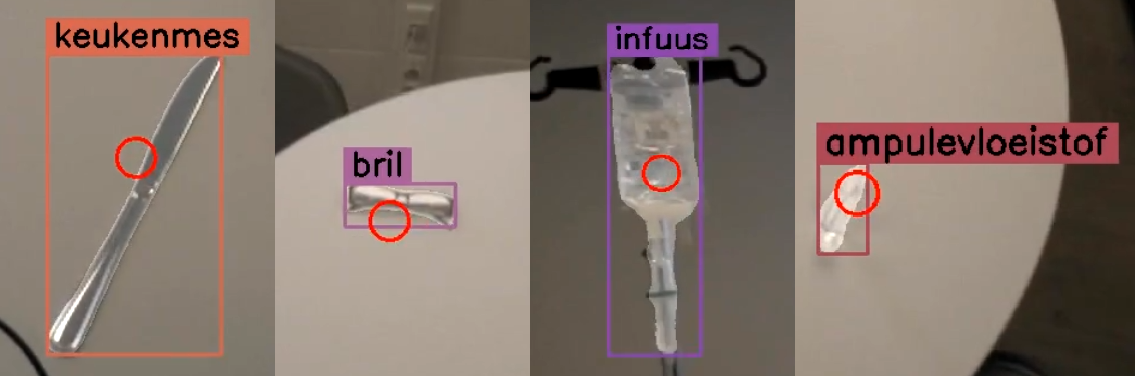
\includegraphics[width=0.8\textwidth]{gaze-overlap.png}
  \caption[]{\label{fig:gaze-overlap} 
    Voorbeelden van de overlap tussen een blikpunt en een segmentatiemasker.
    Indien het blikpunt geheel buiten het masker valt, wordt dit beschouwd als een `niet bekeken' object.
    De rode cirkel stelt het blikpunt voor, met een straal die de fovea en de nauwkeurigheid van de eyetracker modelleert.
  }
\end{figure}

Dit cirkelvormige kijkgebied wordt gedefinieerd op basis van twee principes die in 
Sectie~\ref{sec:fovea-centralis} (Stand van Zaken) werden besproken:
\begin{enumerate}
    \item De fovea centralis, het gebied in het netvlies verantwoordelijk voor het scherpste zicht, beslaat ongeveer 1 graad van het menselijk gezichtsveld.
    \item De nauwkeurigheid van de Tobii Pro Glasses 3 eyetracker, die volgens specificaties ongeveer 0.6 graden bedraagt \autocite{Tobii2025a}.
\end{enumerate}

Om rekening te houden met beide factoren, wordt de effectieve Field of View (FOV) voor 
`aandachtig kijken' benaderd als de som van de foveale FOV en de eyetracker-nauwkeurigheid, dus \(1° + 0.6° = 1.6° \).
Deze gecombineerde hoek wordt vervolgens omgezet naar een pixelradius op het camerabeeld. 
Gegeven de horizontale FOV van de Tobii Pro Glasses 3 camera (95\textdegree, volgens \textcite{Tobii2025a}) en de horizontale resolutie van de video (1920 pixels),
wordt de straal in pixels van het cirkelvormige kijkgebied berekend als:

\[
\text{straal} = \left( \frac{\text{1.6°}}{\text{95°}} \times \text{1920} \right) / 2
\]

Deze waarde maakt de \texttt{mask\_was\_viewed} functie mogelijk, die controleert of het blikpunt van de deelnemer overlapt met een segmentatiemasker.

\begin{listing}[H]
  \begin{minted}{python}
    def mask_was_viewed(
        mask: torch.Tensor,
        gaze_position: tuple[float, float],
        viewed_radius: float = VIEWED_RADIUS,
    ) -> bool:
        # De functie gaat ervan uit dat het masker dezelfde
        # afmetingen heeft als de videoframes (hoogte, breedte).
        # Het blikpunt is een tuple van (x, y) coördinaten.
        # viewed_radius is de straal van de cirkel rond het blikpunt
        height, width = mask.shape
        device = mask.device

        # Creëer een coördinatenrooster voor het masker.
        y_coords = torch.arange(0, height, device=device).view(-1, 1).repeat(1, width)
        x_coords = torch.arange(0, width, device=device).view(1, -1).repeat(height, 1)

        # Bereken het kwadraat van de afstand van elk pixel tot het blikpunt.
        dist_sq = (x_coords - gaze_position[0]) ** 2 + (y_coords - gaze_position[1]) ** 2

        # Creëer een cirkelvormig masker gebaseerd op viewed_radius.
        # Pixels binnen de straal krijgen waarde 1.0, daarbuiten 0.0.
        circular_mask = (dist_sq <= viewed_radius**2).float()
        
        # Pas het cirkelvormige blikmasker toe op het input (segmentatie)masker.
        # Dit gebeurt door een element-wise vermenigvuldiging 
        overlapped_mask = mask * circular_mask

        # Indien de som van de resulterende maskerwaarden groter is dan 0,
        # betekent dit dat er overlap was.
        return bool(overlapped_mask.sum() > 0)

  \end{minted}
  \caption[\texttt{mask\_was\_viewed} functie]{
    Controleert of het blikpunt van de deelnemer overlapt met een segmentatiemasker.
  }
\end{listing}

De werking van deze functie kan als volgt worden samengevat:
\begin{enumerate}
  \item Eerst wordt een binair masker gegenereerd dat het cirkelvormige kijkgebied rond de \texttt{gaze\_position} representeert, 
  gebruikmakend van de berekende\\ \texttt{viewed\_radius}. Pixels binnen deze cirkel krijgen de waarde 1, pixels daarbuiten de waarde 0.
  \item Vervolgens wordt een element-wise vermenigvuldiging uitgevoerd tussen dit binaire kijkgebied-masker 
  en het input segmentatiemasker (dat eveneens binair is, waarbij 1 objectpixels en 0 achtergrondpixels aanduidt). 
  \item Het resultaat is een nieuw masker (\texttt{overlapped\_mask}) dat enkel pixels met waarde 1 bevat waar 
  zowel het oorspronkelijke segmentatiemasker als het cirkelvormige kijkgebied een pixel hadden. 
  Indien de som van alle pixelwaarden in dit \texttt{overlapped\_mask} groter is dan nul, 
  betekent dit dat er ten minste één pixel overlap is, en wordt het object als `bekeken' beschouwd.
\end{enumerate}

\subsection{Bouwen van de Grondwaarheid}

De filtering van de annotaties resulteert in een lijst van bekeken segmentatiemaskers per frame,
wat een directe input vormt voor het construeren van de finale grondwaarheidsdataset.
Voor elke evaluatieopname werden de opgeslagen trackingresultaten 
(de \texttt{.npz}-bestanden, zie Sectie~\ref{sec:labeling-tool-logic}) verder verwerkt. 
Uit elk relevant \texttt{.npz}-bestand werden de volgende kerneigenschappen geëxtraheerd:
\begin{itemize}
  \item De unieke identificatie van de opname (\texttt{recording\_id}).
  \item De index van het videoframe (\texttt{frame\_idx}).
  \item De numerieke ID van het bekeken object (\texttt{class\_id}).
  \item De coördinaten van de bounding box rond het object (\texttt{x1, y1, x2, y2}). Zoals eerder aangegeven, duidt het punt \texttt{(x1, y1)} de linkerbovenhoek aan en \texttt{(x2, y2)} de rechteronderhoek van de bounding box.
  \item De oppervlakte van het segmentatiemasker in pixels (\texttt{mask\_area}), als indicatie van de objectgrootte.
\end{itemize}

Deze gegevens werden samengevoegd tot één tabel, waarbij elke rij een uniek, door een deelnemer bekeken object, 
in een specifiek frame van een evaluatieopname representeert. 
De tabel, opgeslagen als \texttt{data/ground\_truth.csv}, constitueert de finale grondwaarheid.

\subsection{Valideren van de Grondwaarheid}

Om de correctheid van de gegenereerde grondwaarheid te waarborgen, werd een iteratieve, manuele validatiestap uitgevoerd.
Voor elke evaluatieopname werd op elke frame de volgende informatie gevisualiseerd (indien beschikbaar):
\begin{enumerate}
  \item \textbf{Bekeken Objecten:} Voor de objecten die volgens de grondwaarheid in dat specifieke frame als `bekeken' 
  waren geïdentificeerd, werd het bijbehorende segmentatiemasker en een gelabelde bounding box (met objectnaam en -kleur) op het frame getekend.
  \item \textbf{Blikpunt:} Het representatieve blikpunt voor dat frame, werd als een rode cirkel gevisualiseerd.
\end{enumerate}
Deze geannoteerde frames werden vervolgens samengevoegd tot nieuwe video's, opgeslagen in de map \texttt{data/labeling\_validation\_videos}. 

Indien een segmentatiemasker niet correct was (te groot of te klein) of ontbrak (blikpunt op het object, maar geen segmentatie zichtbaar),
ging de onderzoeker terug naar de labeling-tool om dit te corrigeren.
\chapter{Analyse van Observatieprestaties}
\label{ch:analyse}

\section{Inleiding}

In de voorgaande hoofdstukken werden de ontwikkeling van de PoC applicatie, de methodologie voor het verzamelen 
van experimentele data, en het creëren van een grondwaarheidsdataset uitvoerig besproken. 
Dit hoofdstuk richt zich op de kern van het onderzoek: de geautomatiseerde analyse van de 
observatieprestaties van studenten aan de hand van de verzamelde eyetracking-opnames.

Het hoofddoel van de hier beschreven analyse is om, op basis van de videofeed en blikdata van de Tobii Pro Glasses 3, 
automatisch te bepalen (1) welke van de vooraf gedefinieerde kritische objecten door een student zijn waargenomen en (2) 
hoe lang de aandacht op elk van deze objecten gericht was. 
Om dit te realiseren, werd een analysepipeline ontworpen en geïmplementeerd, die de output van verschillende computervisiemodellen combineert.

De ontwikkelde analysepipeline, zoals conceptueel voorgesteld in Strategie 4 van Hoofdstuk~\ref{ch:oplossingsstrategieen}, 
transformeert de ruwe video- en blikdata frame per frame tot een identificatie van bekeken, kritische objecten. 
Dit proces omvat drie hoofdfasen: (1) het segmenteren en tracken van alle potentiële objecten in beeld, 
(2) het filteren van deze segmenten op basis van objectgrootte en daadwerkelijke observatie door de student, en 
(3) het classificeren van de overgebleven objectsegmenten. 
Er worden twee verschillende benaderingen voor de classificatiestap geëvalueerd: één op basis van image embeddings (DINOv2) en een vector-index (Faiss), 
en een tweede die gebruikmaakt van een getraind YOLO-classificatiemodel. 
De prestaties van deze methoden zullen worden beoordeeld aan de hand van de in Hoofdstuk~\ref{ch:grondwaarheid} gecreëerde grondwaarheid.

Figuur~\ref{fig:analyse-pipeline-visualisatie} illustreert de fasen van dit proces aan de hand van illustratieve beelden.

\begin{figure}[H]
    \centering
        \begin{subfigure}[b]{0.75\textwidth}
        \centering
        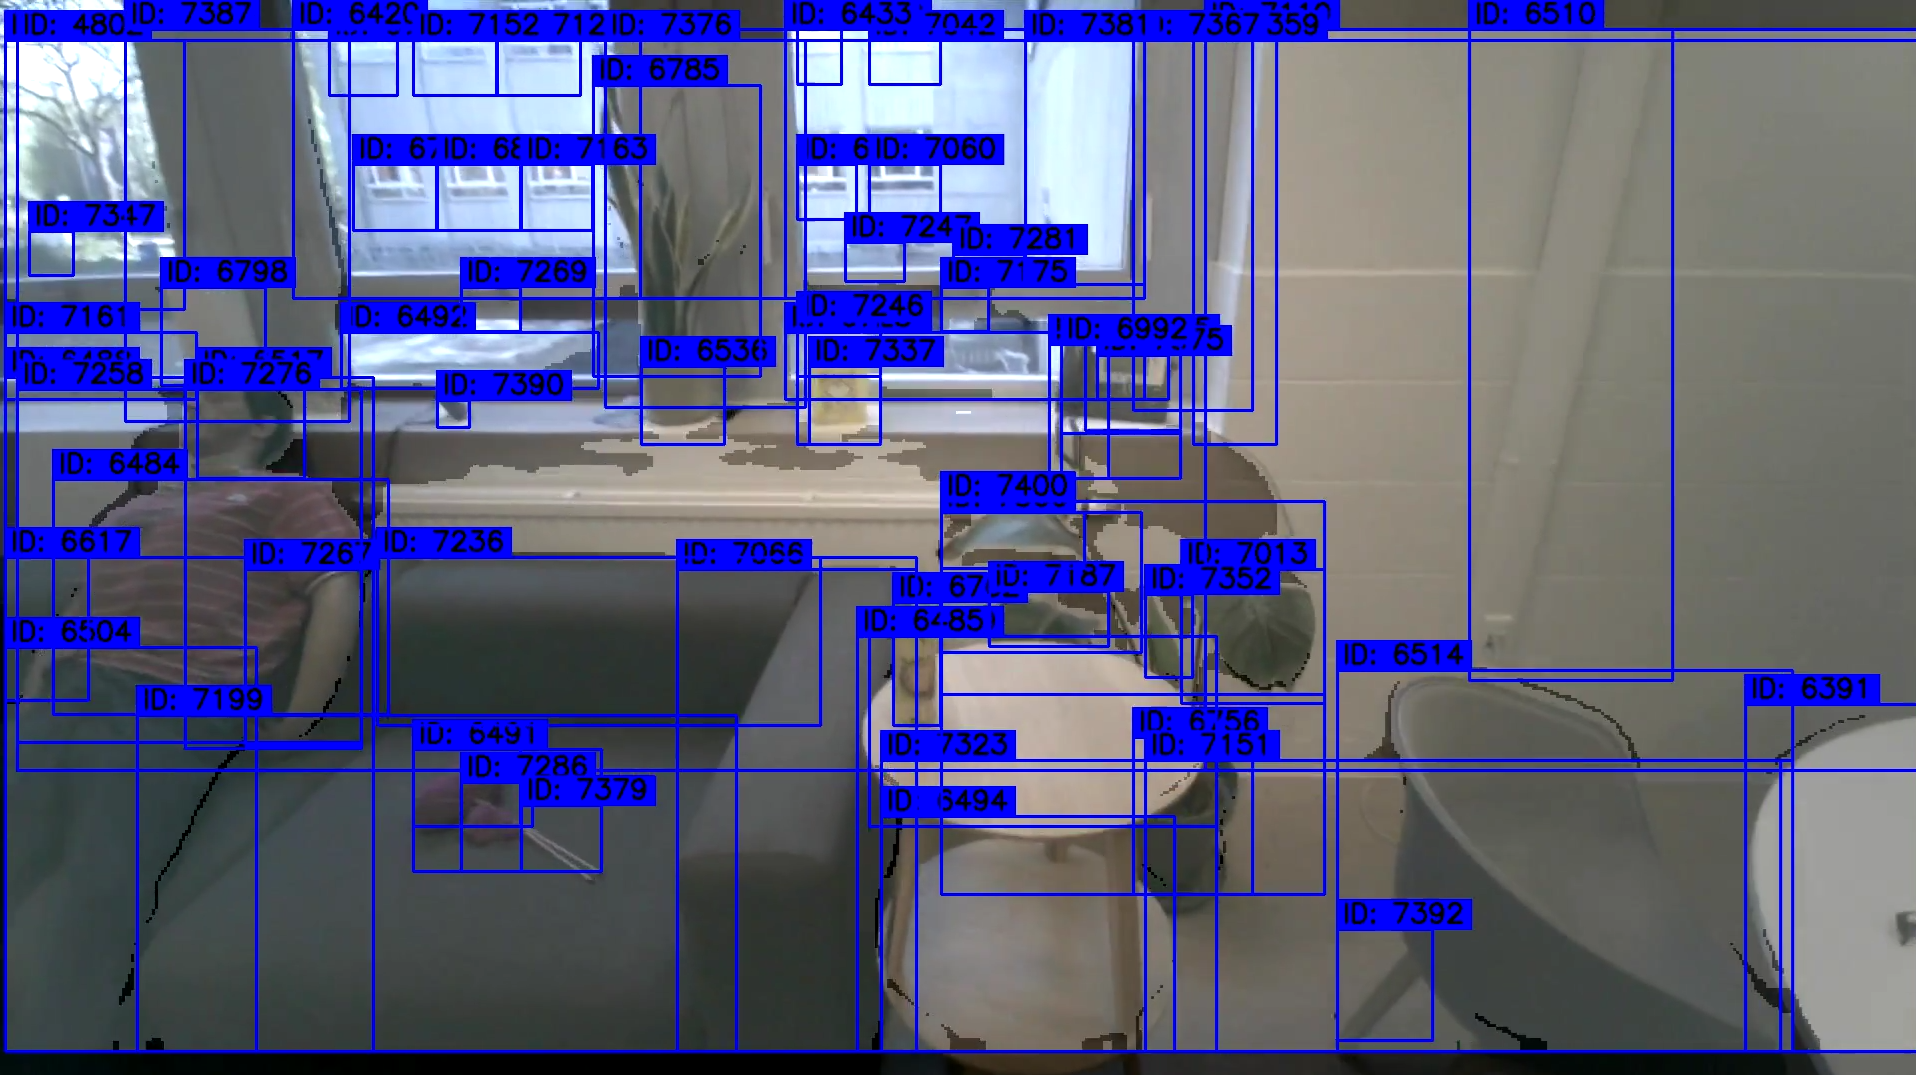
\includegraphics[width=1\textwidth]{everything-prompt.png}
        \caption{Everything-Segmentatie (FastSAM)}
        \label{fig:pipeline_stap_a}
    \end{subfigure}

    \vspace{0.5cm}

    \begin{subfigure}[b]{0.75\textwidth}
    \centering
    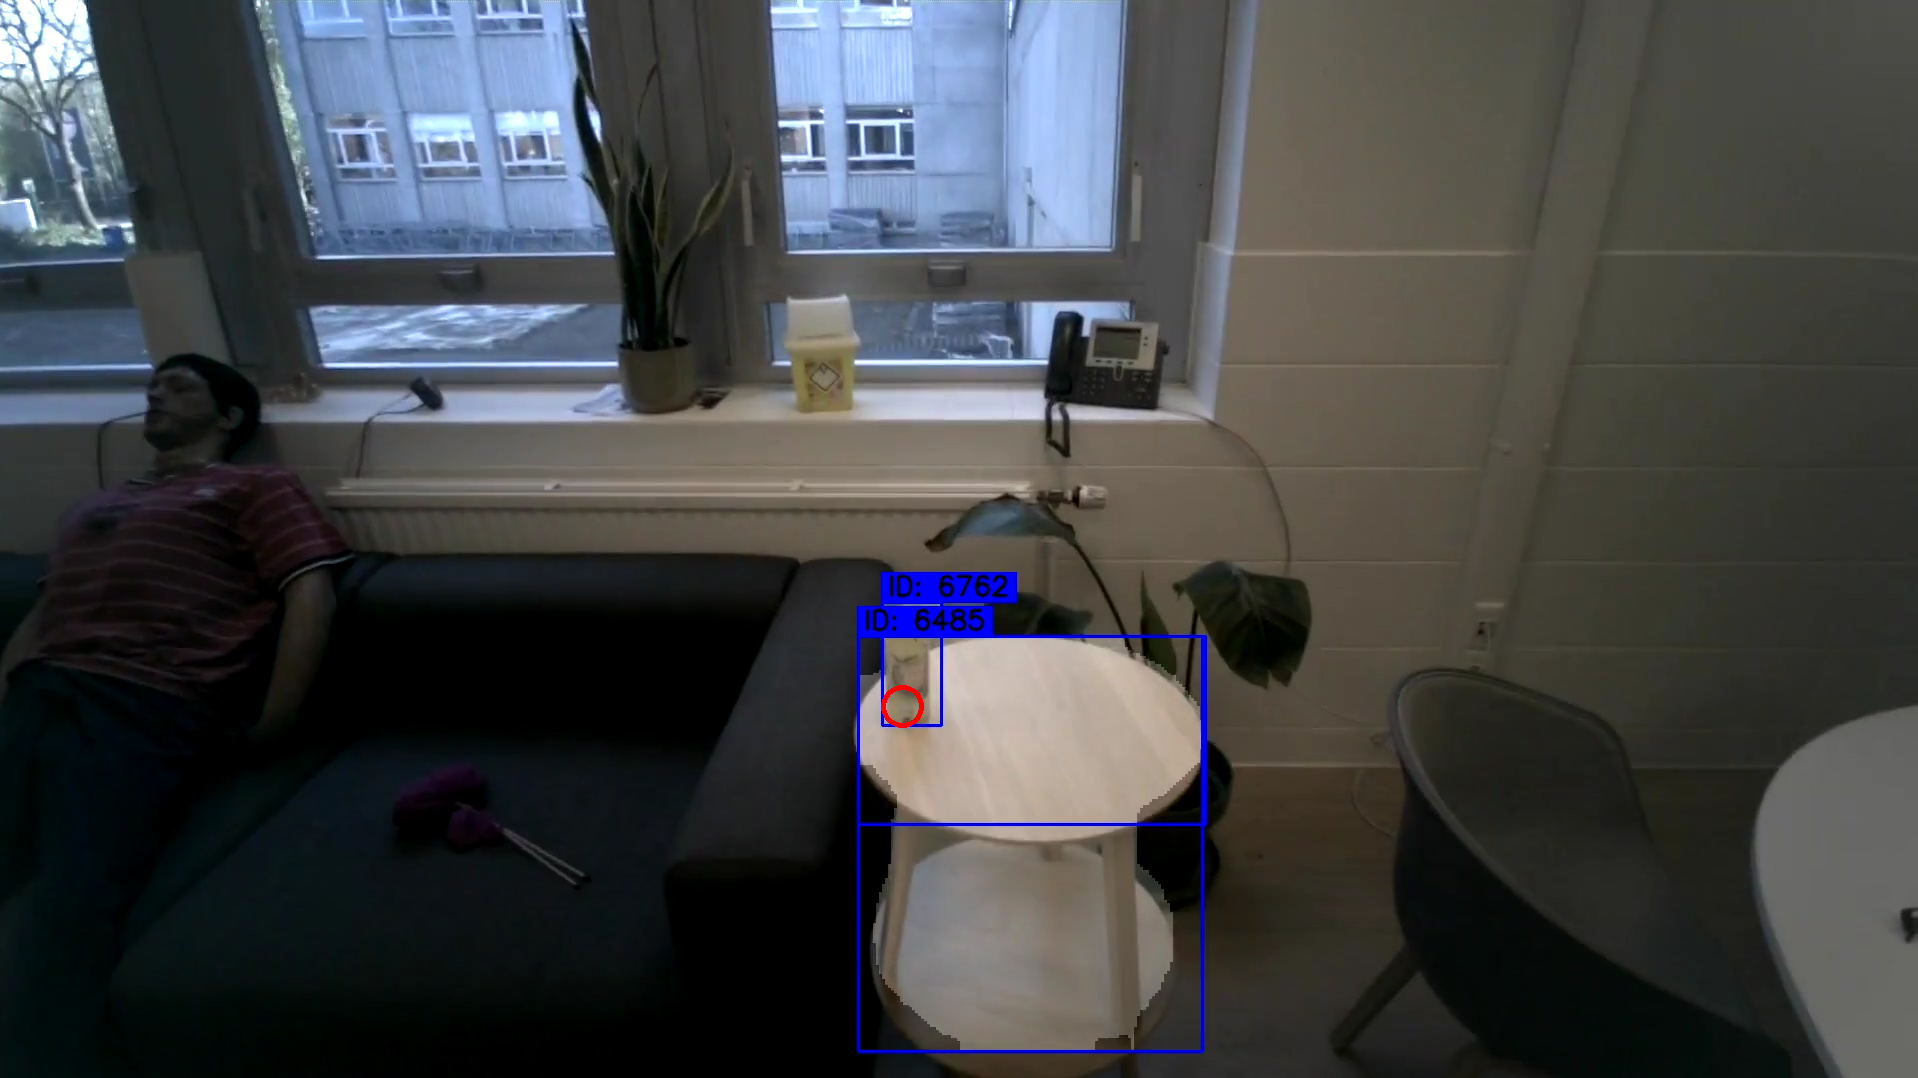
\includegraphics[width=1\textwidth]{filtered-segmentation.png}
    \caption{Filtering op basis van blikpunt en objectgrootte}
    \label{fig:pipeline_stap_b}
    \end{subfigure}

    \vspace{0.5cm}

    \begin{subfigure}[b]{0.75\textwidth}
        \centering
        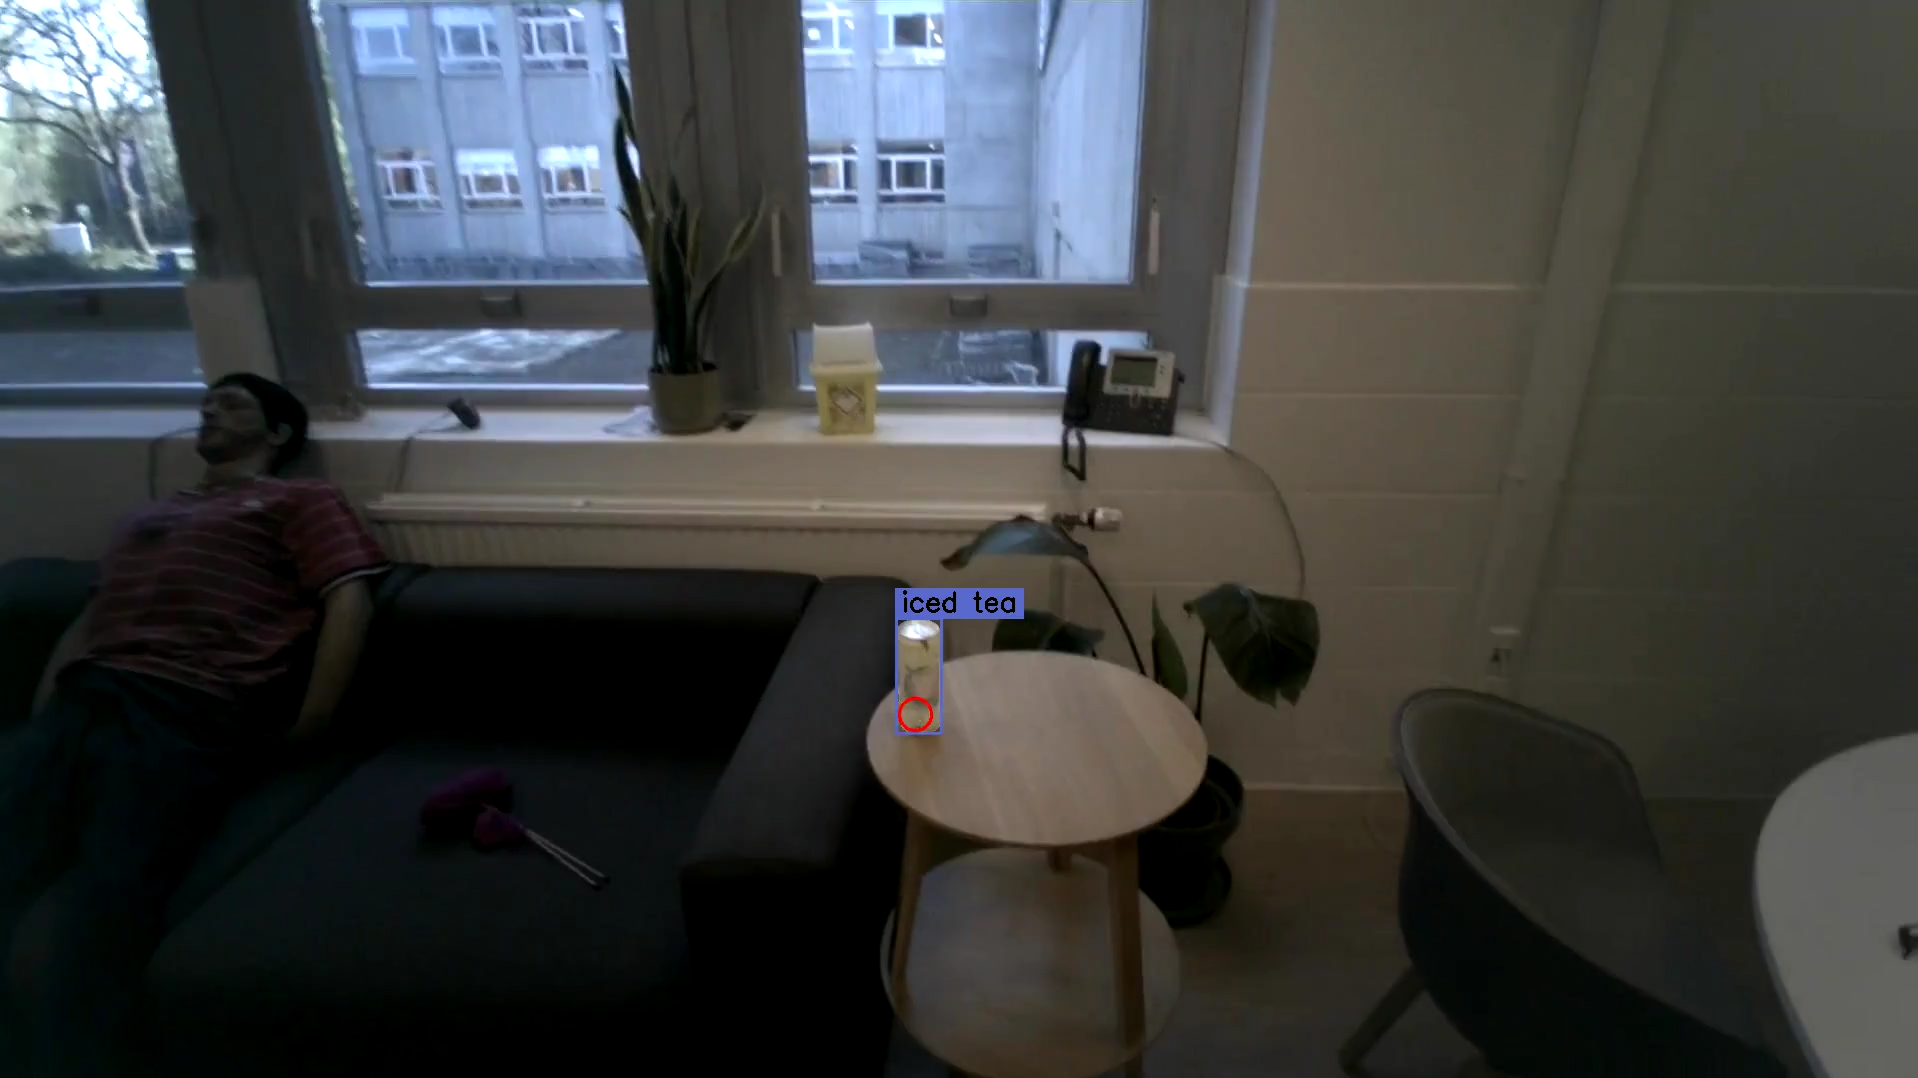
\includegraphics[width=1\textwidth]{classification-example.png}
        \caption{Classificatiestap*}
        \label{fig:pipeline_stap_c}
    \end{subfigure}
    \caption[Visualisatie van de Analysepipeline]{
        \label{fig:analyse-pipeline-visualisatie}
        Visualisatie van de stappen in de analysepipeline.
        (\subref{fig:pipeline_stap_a}) FastSAM identificeert en segmenteert alle potentiële objecten in het frame.
        (\subref{fig:pipeline_stap_b}) De segmenten worden gefilterd; enkel de segmenten die daadwerkelijk met de blik van de gebruiker overlappen worden behouden.
        (\subref{fig:pipeline_stap_c}) De overgebleven segmenten worden uit de originele frame geknipt en dienen als input voor een classificatiemodel.
        *De afbeelding voor de classificatiestap in dit voorbeeld is afkomstig uit een labeling-validatie video.
    }
\end{figure}

\section{Everything-Segmentatie en Objectfiltering}

De eerste fase van de analysepipeline is erop gericht om uit de continue videostroom alle potentieel relevante objectregio's 
te isoleren die daadwerkelijk door de student zijn bekeken. 
De implementatie van dit proces werd vastgelegd in de python-notebook \texttt{04\_gaze\_segmentation.ipynb},
en wordt hieronder toegelicht.
Alle besproken code is te vinden binnen de \texttt{GazeSegmentationJob} klasse in de notebook.

\subsection{Tracking en Segmentatie met FastSAM}

Het FastSAM-model komt in twee varianten: een `large' (\texttt{FastSAM-x}) en een `small' (\texttt{FastSAM-s}) versie.
Hier werd gekozen om de `large' versie te gebruiken, vanwege de betere prestaties in termen van segmentatie en tracking.
Dit model is beschikbaar via de \texttt{ultralytics}\footnote{\url{https://docs.ultralytics.com/models/fast-sam/}} python-bibliotheek,
en bevat een \texttt{track} functie die het mogelijk maakt om alle objecten in een video zowel te segmenteren als te tracken.

\subsubsection{Tracking en Segmentatie van Objecten}

In een eerste stap worden alle frames van de evaluatieopname geëxtraheerd naar een tijdelijke map met behulp van \texttt{ffmpeg}.
Daarna is het mogelijk om de \texttt{track} functie aan te roepen op deze frames:

\begin{listing}[H]
  \begin{minted}{python}
    frame_paths = list(self.frames_path.iterdir())
    # Frames sorteren op basis van hun naam (index)
    frame_paths.sort(key=lambda x: int(x.stem))

    for frame_path in frame_paths:
        frame_idx = int(frame_path.stem)
        results = self.model.track(
            source=str(frame_path), imgsz=1024, verbose=False, persist=True
        )[0]
    \end{minted}
  \caption[Tracking van objecten met FastSAM]{}
\end{listing}

Hier zijn volgende zaken belangrijk om op te merken:
\begin{itemize}
    \item De frames dienen gesorteerd te worden op basis van hun volgorde in de video.
    \item De \texttt{track} functie neemt een parameter \texttt{imgsz} aan, die de grootte van de inputafbeeldingen bepaalt.
    Indien de afbeeldingen te groot of te klein zijn, worden ze automatisch geschaald.
    Deze parameter heeft zowel invloed op de snelheid van de segmentatie als op de kwaliteit ervan.
    \item Het is belangrijk om de \texttt{persist} parameter op \texttt{True} te zetten, 
    zodat het model de tracking-informatie kan behouden tussen opeenvolgende frames.
    \item De \texttt{track} functie retourneert een lijst van \texttt{Results}-objecten maar bevat hier slechts één element.
    Dit \texttt{Results}-object bevat de segmentatiemaskers, bounding boxes, en tracking-informatie voor elk object in het frame.
\end{itemize}

\subsubsection{Filteren van Tracking-Resultaten}

% TODO: wat doen met frames waar geen gazedata is? (objecten kunnen nog steeds nuttig zijn voor classificatie binnen een object-id)

Na het uitvoeren van de tracking en segmentatie, worden de resultaten gefilterd op basis van twee criteria:
\begin{itemize}
    \item \textbf{Objectgrootte:} Segmenten die een onrealistisch groot deel van het beeld beslaan (bijvoorbeeld muren, vloeren, of de gehele achtergrond) worden weggelaten.
    \item \textbf{Blikdata:} Met behulp van de \texttt{mask\_was\_viewed} functie (zie Sectie~\ref{sec:omgaan-met-blikdata}) 
    wordt voor elk overgebleven segment gecontroleerd of het blikveld van de student daadwerkelijk overlapt met het segmentatiemasker in dat specifieke frame. 
    Enkel de `bekeken' segmenten worden behouden voor verdere analyse.
\end{itemize}

Aangezien we het al eerder hebben gehad over de \texttt{mask\_was\_viewed} functie, 
zal hier enkel de \texttt{mask\_too\_large} functie worden besproken:

\begin{listing}[H]
  \begin{minted}{python}
    def mask_too_large(self, mask: torch.Tensor) -> bool:
        MAX_MASK_AREA = 0.1
        height, width = mask.shape
        frame_area = height * width
        max_mask_area = MAX_MASK_AREA * frame_area

        mask_area = mask.sum()
        return mask_area >= max_mask_area
    \end{minted}
  \caption[Filteren van segmenten op basis van grootte]{}
\end{listing}

Hier wordt een som berekend van alle pixels in het segmentatiemasker (aangezien het masker binair is).
Indien deze som groter is dan de maximaal toegestane oppervlakte, wordt het masker als `te groot' beschouwd.
De maximale oppervlakte van een segment wordt gedefinieerd als 10\% van de totale oppervlakte van het frame.
Dit is momenteel een arbitraire waarde, maar kan in de toekomst verder geoptimaliseerd worden, of zelfs 
dynamisch worden ingesteld op basis van objecten binnen kalibratieopnames in de applicatie.

\subsubsection{Opslaan van de Resultaten}

Na het filteren van de segmenten, worden de resultaten opgeslagen in gecomprimeerde numpy-bestanden 
(\texttt{.npz}) onder \texttt{data/gaze\_segmentation\_results}.

\begin{listing}[H]
  \begin{minted}{python}
    executor.submit(
        np.savez_compressed,
        self.results_path / f"{frame_idx}.npz",
        boxes=boxes,
        rois=rois_array,
        masks=masks_array,
        object_ids=object_ids,
        frame_idx=frame_idx,
        gaze_position=gaze_position,
        confidences=confidences,
    )
    \end{minted}
  \caption[Opslaan van segmentatie-resultaten]{}
\end{listing}

De volgende gegevens worden opgeslagen:
\begin{itemize}
    \item \textbf{boxes:} De bounding boxes van de segmenten, handig voor het visualiseren van de segmenten in de video.
    \item \textbf{rois:} De ROI's (Region of Interest) van de segmenten. Deze worden later gebruikt bij de classificatiestap om de objecten te identificeren.
    \item \textbf{masks:} De segmentatiemaskers van de objecten, die ook worden gebruikt voor visualisatie.
    \item \textbf{object\_ids:} De unieke ID's van de objecten, die worden toegewezen door het FastSAM-model.
    \item \textbf{frame\_idx:} De index van het frame, die wordt gebruikt om de resultaten te koppelen aan het juiste frame in de video.
    \item \textbf{gaze\_position:} De blikpositie van de student in dat specifieke frame.
    \item \textbf{confidences:} De vertrouwensscore van het model voor elk segment, die aangeeft hoe zeker het model is dat het segment correct is.
    Dit kan nuttig zijn voor het filteren van segmenten die een lage vertrouwensscore hebben, 
    of het vinden van correlaties tussen de vertrouwensscore en de uiteindelijke classificatie.
\end{itemize}
Aangezien het opslaan van de resultaten IO-intensief is, wordt dit proces uitgevoerd met behulp van multithreading.

\section{Classificatie van Objecten}

\subsection{Voorbereiding van Data voor Classificatie}

De output van de voorgaande fase bestaat uit een reeks \texttt{.npz}-bestanden, één per frame, 
die de gefilterde segmenten, ROIs, en bijbehorende metadata bevatten. 
Om deze data efficiënt te kunnen gebruiken als input voor de classificatiestrategieën, werd een aanvullende voorbereidingsstap uitgevoerd. 
Deze stap werd geïmplementeerd in de notebook \texttt{05\_create\_object\_datasets.ipynb} en consolideert de frame-per-frame 
resultaten tot een gestructureerde dataset per evaluatieopname. 
Deze dataset, hierna "object-dataset" genoemd, vormt de directe input voor zowel de classificatie met een vector-index als de 
classificatie met een YOLO-model.

Het creëren van de object-dataset omvat het itereren over de \texttt{.npz}-bestanden van elke opname. 
Voor elk gedetecteerd en gefilterd object (ROI) binnen een frame worden de volgende kenmerken geëxtraheerd en samengevoegd:
\begin{itemize}
    \item \texttt{frame\_idx}: De index van het frame waarin het object oorspronkelijk werd gedetecteerd. 
    Dit koppelt het object aan een specifiek tijdstip in de video.
    \item \texttt{object\_id}: De unieke, tijdelijke ID die door het FastSAM-model aan het getrackte object 
    is toegewezen binnen de scope van die specifieke tracking-sessie.
    \item \texttt{confidence}: De confidencescore van het FastSAM-model voor de detectie van dit specifieke segment. 
    Deze score geeft een indicatie van hoe zeker het model was van zijn segmentatie.
    \item \texttt{embedding}: Een dense vectorrepresentatie (embedding) van de visuele kenmerken van de ROI, 
    gegenereerd met het DINOv2-model. 
    Deze embedding dient als input voor de op similariteit gebaseerde classificatie met een vector-index.
    Meer hierover in de sectie dat volgt.
    \item \texttt{mask\_area}: De totale oppervlakte van het segmentatiemasker van het object in pixels. 
    Dit geeft een maat voor de (schijnbare) grootte van het object in het frame.
    \item \texttt{x1, y1, x2, y2}: De coördinaten die de bounding box rondom het gedetecteerde object definiëren. 
\end{itemize}

Deze geëxtraheerde informatie wordt per opname samengevoegd in een \texttt{Pandas DataFrame} en vervolgens opgeslagen 
als een \texttt{.csv}-bestand onder \texttt{data/object\_datasets/<recording\_id>}. 
Het resultaat is een set van tabelvormige datasets die klaar zijn voor de daadwerkelijke classificatietaken.
Hoewel veel van deze metadata ook in de individuele \texttt{.npz}-bestanden te vinden is, resulteert de consolidatie 
naar één \texttt{.csv}-bestand per opname in een efficiëntere dataverwerking tijdens de classificatiefase. 
Het vermijdt het herhaaldelijk openen en parsen van potentieel honderden of duizenden afzonderlijke \texttt{.npz}-bestanden.

\subsection{Classificatie met Vector-Index}

TODO

\subsection{Classificatie met YOLO}

TODO


% Voeg hier je eigen hoofdstukken toe die de ``corpus'' van je bachelorproef
% vormen. De structuur en titels hangen af van je eigen onderzoek. Je kan bv.
% elke fase in je onderzoek in een apart hoofdstuk bespreken.

%\input{...}
%\input{...}
%...

%%=============================================================================
%% Conclusie
%%=============================================================================

\chapter{Conclusie}%
\label{ch:conclusie}

% TODO: Trek een duidelijke conclusie, in de vorm van een antwoord op de
% onderzoeksvra(a)g(en). Wat was jouw bijdrage aan het onderzoeksdomein en
% hoe biedt dit meerwaarde aan het vakgebied/doelgroep? 
% Reflecteer kritisch over het resultaat. In Engelse teksten wordt deze sectie
% ``Discussion'' genoemd. Had je deze uitkomst verwacht? Zijn er zaken die nog
% niet duidelijk zijn?
% Heeft het onderzoek geleid tot nieuwe vragen die uitnodigen tot verder 
%onderzoek?

\lipsum[76-80]



%---------- Bijlagen -----------------------------------------------------------

\appendix

\chapter{Onderzoeksvoorstel}

Het onderwerp van deze bachelorproef is gebaseerd op een onderzoeksvoorstel dat vooraf werd beoordeeld door de promotor. Dat voorstel is opgenomen in deze bijlage.

% TODO: 
%\section*{Samenvatting}

% Kopieer en plak hier de samenvatting (abstract) van je onderzoeksvoorstel.

% Verwijzing naar het bestand met de inhoud van het onderzoeksvoorstel
%---------- Inleiding ---------------------------------------------------------

\section{Inleiding}%
\label{sec:inleiding}

Observatievaardigheden van zorgverleners\newline
zijn belangrijk om nauwkeurige diagnoses te stellen
en effectieve zorgplannen te ontwikkelen.
In het 360° Zorglab aan HOGENT worden studenten getraind via simulaties waarbij
hun oogbewegingen worden geregistreerd met Tobii Glasses.
Een belangrijk aspect van deze training is dat studenten leren om kritische objecten,
zoals een colafles op het nachtkastje van een diabetespatiënt, op te merken. 
\par
Hoewel de Tobii Glasses bruikbare eyetracking data leveren, ontbreekt er momenteel geschikte software om te analyseren of studenten daadwerkelijk naar deze objecten hebben gekeken.
Dit gebrek aan dataverwerking en visualisatie maakt het voor trainers lastig om de observatieprestaties van studenten efficiënt te beoordelen en te verbeteren. 
Zonder een geautomatiseerde manier om te detecteren welke specifieke objecten studenten wel of niet hebben waargenomen,\newline wordt het geven van directe feedback een tijdrovend proces.
\par
Om dit probleem aan te pakken, richt dit bachelorproefonderzoek zich op het beantwoorden van de volgende onderzoeksvraag:

\textit{"Hoe kan objectdetectie- en segmentatiesoftware geïntegreerd worden met eyetrackingdata van Tobii Glasses om observatieprestaties van studenten in het 360° Zorglab automatisch te analyseren en te visualiseren?"}

Deze onderzoeksvraag wordt uitgewerkt aan de hand van de volgende deelvragen:
\begin{enumerate}
    \item Welke bestaande objectdetectie en seg- \newline mentatie modellen zijn hiervoor geschikt?
    \item Welke preprocessing- en fine-tuning \newline methoden zijn nodig om Zorglab-specifieke data effectief te gebruiken met deze modellen?
    \item Hoe kan een softwareoplossing ontwikkeld worden voor een gebruiksvriendelijke analyse en visualisatie van eyetrackingdata?
    \item In welke mate kunnen de modellen en de ontwikkelde software een nauwkeurige evaluatie van kritische objectwaarnemingen \newline garanderen?
\end{enumerate}
\par
Het doel is om trainers in het Zorglab te ondersteunen bij het analyseren en visualiseren van deze data, zodat ze snel inzicht krijgen in de observatieprestaties van studenten en kunnen vaststellen of belangrijke objecten tijdens zorgsimulaties zijn waargenomen.

%---------- Stand van zaken ---------------------------------------------------

\section{Stand van zaken}%
\label{sec:literatuurstudie}

\subsection{Bestaande Implementaties}

Recente ontwikkelingen in deep learning hebben de toepassingen van eye-tra\-cking aanzienlijk versterkt, vooral op het gebied van objectdetectie in dynamische en complexe omgevingen.
\par
\textcite{Cho2024} introduceerden het ISGOD systeem, dat oogbewegingen en objectdetectie 
integreert voor kwaliteitsinspectie in productieomgevingen, waarbij real-time analyse mogelijk ge\-maakt wordt ondanks variabele posities en bewegingen. 

\textcite{Cederin2023} onderzochten automatische objectdetectie en tracking in eye tracking analyses en verbeterden de nauwkeurigheid 
door motion deblurring technieken toe te passen, zoals DeblurGAN-v2 gecombineerd met objectdetectoren en trackers. 

Daarnaast combineerde \textcite{Kulyk2023} objectdetectie met eye-tracking data in een virtuele kunsttentoonstelling 
om bezoekersinteresses en visuele aandachtspunten te identificeren. 

\subsection{Machine-learning Modellen}

Naast geïntegreerde eye-tracking systemen, maken de onderzochte studies gebruik van diverse objectdetectiemodellen. 
\par
\textcite{Kulyk2023} maakte gebruik van het Faster R-CNN netwerk, een Convolutioneel Neuronaal Netwerk (CNN) dat 
bekend staat om zijn hoge nauwkeurigheid bij objectdetectie.

\textcite{Cederin2023} breidden hun onderzoek uit door 
naast Faster R-CNN ook andere CNN-gebaseerde architecturen zoals Feature Pyramid Network (FPN), Spatial Pyramid Pooling Network (SPP-Net), 
You Only Look Once (YOLO) en Single Shot MultiBox Detector (SSD) te evalueren. 
Ze onderzochten ook transformer gebaseerde modellen zoals DEtection TRansformer (DETR) en DINO, 
die recentelijk aanzienlijke verbeteringen hebben laten zien in het omgaan met complexe en dynamische scènes.
\par
\textcite{Liu2023} introduceerden in 2023 Grounding DINO, een voorgetraind model dat objecten in afbeeldingen kan detecteren op basis van tekstprompts.
Dit model zou eventueel objecten binnen het Zorglab kunnen detecteren zonder fine-tuning op specifieke data, wat de gebruiksvriendelijkheid van de software zou verbeteren.
\par
Dit bachelorproefonderzoek zal verder gaan dan alleen objectdetectie door ook segmentatiemodellen te verkennen 
die mogelijk via finetuning en tekstprompting specifiek kunnen worden aangepast aan de use case van het 360° Zorglab. 

Een veelbelovend model hiervoor is Meta’s\newline segment Anything Model 2 \autocite{Ravi2024},\newline dat in de medische context succesvol is toegepast door \textcite{Zhu2024}
binnen Medical SAM 2 (MedSAM-2) voor zowel 2D als 3D medische beeldsegmentatie via één enkele prompt. 

\textcite{Wang2023} ontwikkelden GazeSAM, dat eye-tracking 
data gebruikt als inputprompt voor SAM om real-time segmentatiemasks te genereren.

Daarnaast biedt het state-of-the-art werk van \textcite{Bagchi2024} met het ReferEverything framework een model voor het segmenteren van concepten in 
videodata via natuurlijke taal-\newline beschrijvingen, wat relevant kan zijn voor het verwerken van de dynamische videodata van Tobii Glasses.
Momenteel is de code van ReferEverything nog niet beschikbaar, maar de onderzoekers hebben aangegeven dat deze binnenkort open-source zal worden gemaakt.

% Voor literatuurverwijzingen zijn er twee belangrijke commando's:
% \autocite{KEY} => (Auteur, jaartal) Gebruik dit als de naam van de auteur
%   geen onderdeel is van de zin.
% \textcite{KEY} => Auteur (jaartal)  Gebruik dit als de auteursnaam wel een
%   functie heeft in de zin (bv. ``Uit onderzoek door Doll & Hill (1954) bleek
%   ...'')

%---------- Methodologie ------------------------------------------------------
\section{Methodologie}%
\label{sec:methodologie}

De bachelorproef zal worden uitgevoerd\newline volgens een agile aanpak, waarbij iteratieve cycli (sprints) 
en overlappende fasen worden gebruikt om flexibiliteit en continue verbetering mogelijk te maken. 
Deze aanpak zorgt ervoor dat verschillende onderdelen van het project parallel kunnen verlopen en snel 
kunnen worden aangepast op basis van tussentijdse bevindingen. Nieuwe taken worden doorheen de sprints toegevoegd 
aan een backlog binnen een Trello-bord, en worden doorheen de sprints opgepakt en afgerond.
\par
Het doel voor de PoC is om een user-flow te ontwikkelen die het mogelijk maakt om de volgende zaken uit te voeren:
\begin{itemize}
    \item 1. Het ophalen van eyetrackingdata van de Tobii Glasses
    \item 2. Het definiëren van kritische objecten die geobserveerd moeten worden.
    \item 3. Het analyseren van van de data met\newline objectdetectie- en segmentatiemodellen.\newline
    Deze stap wordt hierna de data-architectuur genoemd.
    \item 4. Het al dan niet manueel wegfilteren van vals-positieve objectdetecties.
    \item 5. Het visualiseren van de resultaten van de analyse via een metriek die de blik-punten van de studenten koppelt aan de gedetecteerde objecten.
\end{itemize}
\par
De voorkeur gaat naar het gebruik van voorgetrainde modellen om de nood aan hertrainen te minimaliseren en zo de gebruikerservaring te verbeteren.
Indien nodig kan de PoC uitgebreid worden met extra functionaliteiten zoals het finetunen van modellen met simulatiespecifieke data.

%---------- Tijdsplanning ------------------------------------------------------
\section{Tijdsplanning}
De bachelorproef is gepland van 10 februari 2025 tot en met 23 mei 2025, met een totaal van 7 sprints van 2 weken.
De activiteiten binnen elke sprint omvatten, in geen specifieke volgorde:
\begin{itemize}
    \item Literatuurstudie
    \item Dataverzameling en labeling
    \item Modelselectie en implementatie
    \item Schrijven van Python Notebooks voor experimenten
    \item Ontwikkelen van de data-architectuur binnen de PoC
    \item Ontwikkelen van de user interface voor de PoC
    \item Uitbreiding van de PoC met nieuwe functionaliteiten
    \item Unit-testen schrijven voor de PoC
    \item Meetings met de co-promotor voor\newline feedback en verfijning van de oplossing
    \item Documentatie van het proces en resultaten
    \item Uitschrijven, aanpassen van het proefschrift
\end{itemize}
\par
De onderstaande tijdsplanning geeft een overzicht van de beoogde deliverables en mijlpalen per sprint.
\begin{itemize}
    \item \textbf{Sprint 1}
        \begin{itemize}
            \item Relevante modellen zijn verzameld en uitgetest binnen een Python Notebook.
            \item Er zijn huisgemaakte data verzameld via geleende Tobii Glasses uit het Zorglab.
            \item Potentiële segmentatie- en detectiepipeline architecturen voor de PoC zijn uitgestippeld.
            \item Er is een user interface binnen de PoC om opnames op te halen van de Tobii Glasses.
        \end{itemize}
    \item \textbf{Sprint 2}
        \begin{itemize}
            \item Er is zorglab-specifieke data\newline aangevraagd.
            \item De abstract en inleiding van het proefschrift zijn geschreven.
            \item Het literatuurstudie onderdeel van het proefschrift is uitgewerkt.
        \end{itemize}
        \item \textbf{Sprint 3}
        \begin{itemize}
            \item Er is een demo gegeven aan de\newline co-promotor voor een kandidaat\newline architectuur van de PoC.
            \item De feedback van de co-promotor is verwerkt en gedocumenteerd.
            \item Er is een metriek ontwikkeld voor het meten van waar een student naar heeft gekeken en voor hoe lang.
            \item Er zijn verschillende data-architecturen geëvalueerd.
        \end{itemize}
    \item \textbf{Sprint 4}
        \begin{itemize}
            \item De segmentatie- en detectiepipeline is geïntegreerd binnen de user interface van de PoC
            \item De vergelijking tussen verschillende\newline data-architecturen is toegevoegd aan\newline het proefschrift.
            \item Er is een meeting gebeurd met de co-promotor voor feedback op de PoC.
        \end{itemize}
    \item \textbf{Sprint 5}
        \begin{itemize}
            \item De objectdetectie- en segmentatiemodellen zijn geïntegreerd binnen de PoC.
            \item Zorglab-specifieke data is gelabeld en gebruikt voor het valideren van de PoC.
        \end{itemize}
    \item \textbf{Sprint 6}
        \begin{itemize}
            \item De visualisatie-interface is ontwikkeld\newline en geïntegreerd binnen de PoC.
            \item De gebruiker kan nieuwe video's analyseren en de resultaten bekijken.
            \item De PoC is gevalideerd in het Zorglab.
        \end{itemize}
    \item \textbf{Sprint 7}
        \begin{itemize}
            \item Het proefschrift is gefinaliseerd en ingediend.
        \end{itemize}
\end{itemize}

%---------- Tools en Technologieën ----------------------------------------------
\subsection{Tools en Technologieën}

\begin{itemize} 
  \item \textbf{Programmeertaal en Frameworks}: Python, PyTorch, TensorFlow voor\\ machine-learning modellering en implementatie. 
  \item \textbf{Programmeerstack van de PoC}: FastAPI\newline voor de backend, HTMX en Jinja2 voor de frontend.
  \item \textbf{Data Verwerking en Visualisatie}: OpenCV voor videoverwerking, Matplotlib voor datavisualisatie. 
  \item \textbf{Ontwikkelomgeving}: Visual Studio Code,\newline Python Notebooks voor experimenten, Git voor versiebeheer. Poetry voor dependency management.
  \item \textbf{GPU}: At-home Nvidia RTX 4090 en eventuele GPUs van HoGent.
  \item \textbf{Eyetracking}: Tobii Eyetracking Glasses, en Tobii Pro Glasses 3 Controller App.
  \item \textbf{Planning}: Trello voor projectmanagement.
\end{itemize}

%---------- Verwachte resultaten ----------------------------------------------
\section{Verwacht resultaat}%
\label{sec:verwachte_resultaten}

Het verwachte resultaat van dit bachelorproefonderzoek is de ontwikkeling van een functionele PoC 
software die objectherkennings- en segmentatiemodellen integreert met de videodata van de Tobii Eyetracking Glasses.
Deze software zal in staat zijn om nauwkeurig te bepalen welke kritische objecten door studenten zijn waargenomen tijdens simulaties, 
ondersteund door visuele representaties van de oogbewegingen. Verwacht wordt dat modellen na fine-tuning met Zorglab-specifieke data, 
een hoge detectienauwkeurigheid zullen bereiken.
\par
Trainers en lesgevers in het 360° Zorglab, zullen baat hebben bij een efficiëntere en gedetailleerdere 
evaluatie van de observatieprestaties van studenten. De ontwikkelde software biedt een meerwaarde door het mogelijk 
te maken gerichte feedback te geven op specifieke waarnemingen, waardoor het leerproces wordt geoptimaliseerd. 
Bovendien draagt de PoC bij aan de verdere automatisering van het beoordelingsproces, wat leidt tot tijdbesparing. 
Het onderzoek zal ook inzicht bieden in de effectiviteit van verschillende 
machine-learning modellen binnen de context van eyetrackingdata, wat kennis oplevert voor toekomstige toepassingen en verbeteringen in het Zorglab.

\appendix 

\chapter{Best-practices voor het werken met de Tobii Pro Glasses 3}
\label{ch:best-practices}

TODO

% TODO: Dit hoofdstuk bevat een samenvatting van de best-practices voor het werken met
% de Tobii Pro Glasses 3, en andere interessante opmerkingen die gemaakt werden tijdens de bachelorproef.


%%---------- Backmatter, referentielijst ---------------------------------------
\backmatter{}

\setlength\bibitemsep{2pt} %% Add Some space between the bibliograpy entries
\printbibliography[heading=bibintoc]

\end{document}
